% !TeX root = main.tex
\documentclass[12pt]{report} % font: 12pt

% margins: 2.5 cm top and bottom; 3 cm left and right
\usepackage[
a4paper,
vmargin=2.5cm,
hmargin=3cm
]{geometry}

% Paragraph Spacing and Line Spacing: Narrow (6 pt / 1.15 spacing) or Moderate (6 pt / 1.5 spacing)
\renewcommand{\baselinestretch}{1.15}
\parskip=6pt

% Color settings for cover and code listings 
\usepackage[table]{xcolor}
\definecolor{azulUC3M}{RGB}{0,0,102}
\definecolor{gray97}{gray}{.97}
\definecolor{gray75}{gray}{.75}
\definecolor{gray45}{gray}{.45}
\usepackage[ruled,vlined,linesnumbered]{algorithm2e} % For algorithms
\usepackage{forest}

% PDF/A -- Important for its inclusion in e-Archive. PDF/A is the optimal format for preservation and for the generation of metadata: http://uc3m.libguides.com/ld.php?content_id=31389625. 

% In the template we include the file OUTPUT.XMPDATA. You can download that file and include the metadata that will be incorporated into the PDF file when you compile the memoria.tex file. Then upload it back to your project.  
\usepackage[a-1b]{pdfx}
\usepackage{datetime} % DATETIME
\newdateformat{monthyeardate}{%
  \monthname[\THEMONTH], \THEYEAR}
% LINKS
\usepackage{hyperref}
\hypersetup{colorlinks=true,
	linkcolor=black, % links to parts of the document (e.g. index) in black
	urlcolor=blue} % links to resources outside the document in blue

% MATH EXPRESSIONS
\usepackage{amsmath,amssymb,amsfonts,amsthm,amsgen}

% Character encoding
\usepackage{txfonts} 
\usepackage[T1]{fontenc}
\usepackage[utf8]{inputenc}

% English settings
\usepackage[english]{babel} 
\usepackage[babel, english=american]{csquotes}
\AtBeginEnvironment{quote}{\small}

% Footer settings
\usepackage{fancyhdr}
\pagestyle{fancy}
\fancyhf{}
\renewcommand{\headrulewidth}{0pt}
\rfoot{\thepage}
\fancypagestyle{plain}{\pagestyle{fancy}}

% DESIGN OF THE TITLES of the parts of the work (chapters and epigraphs or sub-chapters)
\usepackage{titlesec}
\usepackage{titletoc}
\titleformat{\chapter}[block]
{\large\bfseries\filcenter}
{\thechapter.}
{5pt}
{\MakeUppercase}
{}
\titlespacing{\chapter}{0pt}{0pt}{*3}
\titlecontents{chapter}
[0pt]                                               
{}
{\contentsmargin{0pt}\thecontentslabel.\enspace\uppercase}
{\contentsmargin{0pt}\uppercase}                        
{\titlerule*[.7pc]{.}\contentspage}                 

\titleformat{\section}
{\bfseries}
{\thesection.}
{5pt}
{}
\titlecontents{section}
[5pt]                                               
{}
{\contentsmargin{0pt}\thecontentslabel.\enspace}
{\contentsmargin{0pt}}
{\titlerule*[.7pc]{.}\contentspage}

\titleformat{\subsection}
{\normalsize\bfseries}
{\thesubsection.}
{5pt}
{}
\titlecontents{subsection}
[10pt]                                               
{}
{\contentsmargin{0pt}                          
	\thecontentslabel.\enspace}
{\contentsmargin{0pt}}                        
{\titlerule*[.7pc]{.}\contentspage}  


% Tables and figures settings
\usepackage{multirow} % combine cells 
\usepackage{caption} % customize the title of tables and figures
\usepackage{floatrow} % we use this package and its \ ttabbox and \ ffigbox macros to align the table and figure names according to the defined style.
\usepackage{array} % with this package we can define in the following line a new type of column for tables: custom width and centered content
\newcolumntype{P}[1]{>{\centering\arraybackslash}p{#1}}
\DeclareCaptionFormat{upper}{#1#2\uppercase{#3}\par}
\usepackage{graphicx}
%\graphicspath{{Include/imagenes/}} % Images folder

% Table layout for engineering
\captionsetup*[table]{
	format=upper,
	name=TABLE,
	justification=centering,
	labelsep=period,
	width=.75\linewidth,
	labelfont=small,
	font=small
}

% Figures layout for engineering
\captionsetup[figure]{
	format=hang,
	name=Fig.,
	singlelinecheck=off,
	labelsep=period,
	labelfont=small,
	font=small		
}

% FOOTNOTES
\usepackage{chngcntr} % continuous numbering of footnotes
\counterwithout{footnote}{chapter}

% CODE LISTINGS 
% support and styling for listings. More information in  https://es.wikibooks.org/wiki/Manual_de_LaTeX/Listados_de_código/Listados_con_listings
\usepackage{listings}

% Custom listing
\lstdefinestyle{estilo}{ frame=Ltb,
	framerule=0pt,
	aboveskip=0.5cm,
	framextopmargin=3pt,
	framexbottommargin=3pt,
	framexleftmargin=0.4cm,
	framesep=0pt,
	rulesep=.4pt,
	backgroundcolor=\color{gray97},
	rulesepcolor=\color{black},
	%
	basicstyle=\ttfamily\footnotesize,
	keywordstyle=\bfseries,
	stringstyle=\ttfamily,
	showstringspaces = false,
	commentstyle=\color{gray45},     
	%
	numbers=left,
	numbersep=15pt,
	numberstyle=\tiny,
	numberfirstline = false,
	breaklines=true,
	xleftmargin=\parindent
}

\captionsetup*[lstlisting]{font=small, labelsep=period}
 
\lstset{style=estilo}
\renewcommand{\lstlistingname}{\uppercase{Código}}


% REFERENCES 

% IEEE bibliography setup
\usepackage[backend=biber, style=ieee, isbn=false,sortcites, maxbibnames=6, minbibnames=1]{biblatex} % Setting for IEEE citation style, recommended for engineering. "maxbibnames" indicates that from 6 authors truncate the list in the first one (minbibnames) and add "et al." as used in the IEEE style.

\addbibresource{References.bib} % The references.bib file in which the bibliography used should be



% Para nuestros teoremas,corolarios, lemas etc...
\newtheoremstyle{break}
{\topsep}{\topsep}%
{\selectfont}{}%
{\bfseries}{}%
{\newline}{}%

\theoremstyle{break}
\newtheorem{theorem}{Theorem}[section]
\newtheorem{lemma}[theorem]{Lemma}
\newtheorem{caracterization}[theorem]{Caracterization}
\newtheorem{property}[theorem]{Property}
\newtheorem{proposition}[theorem]{Proposition}
\newtheorem{corollary}[theorem]{Corollary}
\newtheorem{Conjecture}[theorem]{Conjecture}
\newtheorem{example}[theorem]{Example}
\newtheorem*{remark}{Remark}
\newtheorem*{notation}{Notation}
\newtheorem{definition}[theorem]{Definition}

% Fecha

\usepackage{csvsimple}

  


\newcommand{\AuthorsName}{Fernando Bellido Pazos}
\newcommand{\Tutor}{Juan Manuel Pérez Pardo}


\newcommand{\Edu}{Applied and Computational Mathematics}
\newcommand{\Where}{Universidad Carlos III de Madrid}


\newcommand{\Title}{BNumMet} 
\newcommand{\Subtitle}{A Scholar implementation of Numerical Methods in Python enhanced with interactive widgets}




\newcommand{\Fecha}{\monthname, \the\year } % Not Working \monthyeardate


\begin{document}
\pagenumbering{roman} % Roman numerals are used in the numbering of the pages preceding the body of the work.

% Cover
\input{Include/Cover}


\newpage % blank page
\thispagestyle{empty}
\mbox{}

% 0. Abstract
\renewcommand\abstractname{\large\bfseries\filcenter\uppercase{Summary}}
\begin{abstract}
	\thispagestyle{plain}
	\setcounter{page}{3}

	% Write your abstract
	\newcommand{\KeywordsAbstract}{Numerical methods, Open-source, Python, Jupyter, Software development, Linear systems, Interpolation, Nonlinear, Least squares, Random number generators}

The presented end of master's thesis provides an open-source Python package (BNumMet) that gives an academic implementation of the numerical methods taught in universities, as well as a graphical user interface over the Jupyter Notebooks framework, all with the intention of assisting students in their learning of the various numerical methods; it also serves as a tool for professors to assist students in learning these methods.


In this project, we discuss whether previous work in this field has been done, how the project was carried out, what the fundamental criteria for this project are, what the underlying algorithms are, and whether the solutions proposed are both efficient, comprehensible, and doable for students.

Overall, this project can be used as a model for the development of didactic tools in the scientific community in order to increase the number of people who enter the S.T.E.M. (Science, Technology, Engineering, and Mathematics) fields and make the learning and studying of methods that are widely used in the scientific community more intuitive. 

	\textbf{Keywords:  \KeywordsAbstract} % add the keywords

	\vfill
\end{abstract}
\newpage % Blank page
\thispagestyle{empty}
\mbox{}


\chapter*{Dedication}

\setcounter{page}{5}
% Write here	
For a total of 5 years, I have been expanding my knowledge in Mathematics and Computer Science in higher levels of education, not only was my journey full of ups and downs but also with outstanding people that made these highs and lows worth every moment. 

To say 'thank you' would only be an understatement of my true appreciation to these people who have been with me and, I hope, will always be on this journey of enlightenment. To such an extent, I want to give all the credit to the ones that provided me with the chance to find new objectives in life, and who always pushed me to strive to be my best self in every aspect of life, that credit is in large part to both my Mother, Maria Pazos Arenal, and Father, Fernando Bellido Alonso-Carriazo as well as all the members of my family to whom I owe a large part of my very best moments.

I would like to extend my greatest and deep appreciation to my best colleagues who made me laugh even in the darkest of times, my outstanding music group at \textit{Sol Menor} that allowed me to express beyond the academic, see beyond reason by expressing and understanding music and teaching me about what team-work really means.

In addition, I want to express my most sincere thank you to my tutor Juan Manuel Pérez Pardo who has accompanied me through the development of this work as well as the teachers who once pushed me to strive towards the study of Science, those being Concha Elena Alegre, María Pilar Cuesta López, Aurora Insua Ruíz and my other fellow teachers and professors.
\quote{
\textit{One looks back with appreciation to the brilliant teachers, but with gratitude to those who touched our human feelings} - Carl Gustav Jung \cite{Jung+1954}
}
\vfill
\newpage % blank page
\thispagestyle{empty}
\mbox{}


\tableofcontents % Table of contents
\thispagestyle{fancy}
\newpage % blank page
\thispagestyle{empty}
\mbox{}

%--
% List of figures. If they are not included, comment the following lines
%-
\listoffigures
\thispagestyle{fancy}
\newpage % blank page
\thispagestyle{empty}
\mbox{}

%--
% List of tables. If they are not included, comment the following lines
%-
\listoftables
\thispagestyle{fancy}
\newpage % blankpage
\thispagestyle{empty}
\mbox{}

%--
% List of Algorithm. If they are not included, comment the following lines
%-
\listofalgorithms
\thispagestyle{fancy}
\newpage % blankpage
\thispagestyle{empty}
\mbox{}
\clearpage
\pagenumbering{arabic} % numbering with Arabic numerals for the rest of the document.


% 2. Introduction
\chapter{Introduction}

Ever since the development of the brain, we humans have been developing various tools and techniques that provided some “evolutionary” benefit, let that be the wheel, fire, hunting weapons and all sorts of machinery to make both our life easier and/or have an advantage over something. 
Around the Second World War, we started to envision a world of computers, machines that will allows us to handle repetitive processes and make calculations that otherwise would take a lot of resources to be carried out. This technological evolution involved a change of mindset in the mathematical world, machines - now - could potentially make the more tedious and cumbersome calculations in a short span of time, in contrast to what it has been done until then, by mere handmade calculations, and the area of – what we now call –Numerical methods/Analysis was just starting to get its popularity.


It is imperative to acknowledge that until the rise of the computers, numerical methods/analysis has been in a never-ending development and used in a large scale, to name a few:
\begin{enumerate}
    \item Calculation of logarithms
    \item Interpolation
    \item Finding zeros of a function (Newton's Method)
    \item Finite Differences
    \item Least Squares Problem
    \item Quadrature rules
\end{enumerate}

For a more detailed view on this history, I refer you to \cite{goldstine2012history}. The methods mentioned are only the tip of the iceberg and provided, in some cases, solutions to problems that could only be formulated and not solved using analytical approaches. 
The impact of computers and numerical approaches combined during its birth can only be grasped, and ever since J. Von Neumann the world started to shift towards a computerized mathematical realm.


Nowadays, we have powerful enough computers that take these numerical methods and solve most of these problems, to such extend that even a 6 inch smartphone can perform a vast number of calculations that on the 20th century could have taken years, but there is one dilemma we still face, how can we teach the future generations these methods in such a way that they find it as natural and intuitive as adding or subtracting? Pondering on the question, one could argue that the sudden rise of technology implies we must try to always be at the verge of what our current technological capabilities are, and how can we extrapolate this knowledge to continue moving forward with this avalanche of improvements, but it is clear that this does not solve the main problem of education.


This end of master thesis aims to give an answer to this dilemma, providing both student and professors a framework that contains the Scholarly version of the well-known numerical methods developed, using the latest, more popular, economical, easy-to-read, and well-known programming language whilst also granting the ability to see how the algorithms work visually.  


% 3. Thesis
\chapter{State of the Art}
\section{Mathworks}
The underlying idea behind this project comes from~\cite{doi:10.1137/1.9780898717952} in which the author, Cleve Moller, provides a textbook for students to get an introduction to numerical methods using Matlab; not only does this work provide with the guide to understand the fundamental numerical methods, but it also includes attached the code for the various methods he includes, while also creating a Graphical User Interface for each method to help students gain a better understanding of such. The code is written in Matlab, which is a proprietary programming language developed by Mathworks, Inc. and is widely used in the scientific community.

Mathworks has created a series of packages that are freely available to the public. These packages are known as Toolboxes, and they may be downloaded from the Mathwork's website. 

Along with the graphical interface, the author created some of the following chapters and the visualization associated:
\begin{itemize}
    \item Linear Equations: LU Decomposition Visualizer
    \item Interpolation: Visualization of various interpolation techniques
    \item Zeros and Roots: Brent-Dekker's Algorithm visualizer
    \item Least Squares: Applying least squares to the US Census 
    \item Quadrature: Visualization of how quadrature applies
    \item Ordinary Differential Equations: How different finite difference schemes work
    \item Fourier Analysis: Visualization of Fourier Analysis
    \item Random Numbers: Some simple Random Number Generators
    \item Eigenvalues and Singular Values: Visualization on how they are obtained from the matrix
\end{itemize}



\subsection{Author comments on this work}
Although C. Moller provides the initial framework for solving the main dilemma we are faced with, there are potential improvements that could be made to the project, among them, the following are proposed:

\begin{enumerate}
    \item Make use of a programming language that is open-source and free to use while also one that is widely used in the scientific community, in the industry as well as being one that should be popular amongst programmers, this fact will allow for the project to be more accessible and future-proof.
    \item Provide an Open Source Licence for the project to be used and improved by anyone while also giving the authors the credit they deserve.
    \item Provide a more intuitive and user-friendly Graphical User Interface that is also more aesthetically appealing.
\end{enumerate}


Overall, the work done by C. Moller is a great starting point for the development of this project, but it is not enough to solve the dilemma presented in the Introduction, since it is not open source and it is not free to use and therefore, it is not accessible to everyone to either use or improve. Additionally, it is built on a less popular programming language, according to the TIOBE Index~\cite{tiobe}.


\section{End-of-Degree Thesis}
One of the attempts to solve the dilemma presented in the Introduction was first tackled by Juan Camilo Bucheli and Juan Manuel Pérez Pardo, as an end-of-degree thesis,~\cite{bucheli2020}. Together, they constructed the first framework for the underlying idea behind BNumMet.
They carefully went over the details of the Socio-Economical front and development of the project, and they also discussed both the meaning of what it means for a project to be open source and the licences associated with them. Additionally, they pondered on the reasons of their choice of the programming language and discussed the main and widely-used library of numerical methods (LAPACK).

The authors implemented the Linear Systems Chapter in this project, prioritizing the LU decomposition with Matlab's translation of the LU Decomposition visualizer. They also began developing the Interpolation visualizer using some of the interpolation methods mentioned in the work from Mathworks.

It should be emphasized that the numerical techniques applied are not licensed; they are open-source, with the exception of some tolerance considerations and step selection; the only thing licensed are the visualizers for each chapter.


\subsection{Author comments on this work}
After a closer investigation of the project, we must ask the following questions that derive from this work.
\begin{enumerate}
    \item Is the licence they had previously chosen still valid with the current evolution of technology?
    \item Is Python still the best programming language for these sort of goals?
    \item Can we improve the global state of the art?
    \item Is the previously done code valid and/or useful for continuing the work?
    \item How can we continue the work as the author would have wanted?
    \item Are the principles of open source followed?
\end{enumerate}

Even though the code they provided is readable and fairly functional, there exists room for improvement, on the one hand the code must be translated to the English language; reasons vary from being the universal language of coding to the fact that is the most spoken language in the world, thereby enabling access to this project to a vast majority of people. On the other hand, the overall algorithmic could be improved. The following list enumerates some of the weak points behind their project:

\begin{enumerate}
    \item The use of threading on the LU Graphical User interface can be simplified to not use threading to reduce computer resources as well as improving the readability of the project.
    
    This raises a few problems such as being more cumbersome to read, understand, maintain and improve. A possible solution is to study carefully the underlying theory of the LU decomposition and then apply it to the code to remove the threading, thereby improving the code. 
    \item Naming and code conventions to current Python standards.
    
    This is important because it allows for the code to be more readable and understandable by other programmers. To do this, we must use the different tools that other programmers have created to help us follow the conventions, such as Pylint, Pydocstyle, Flake8, Sonarqube, etc.

    \item An overall improvement on how the tests are made.
    
    The overall testing of the J.C. Bucheli's code is not as good as it could be, it only checks the overall functionality of the code and not the extreme cases that the algorithm has, something which breaks with the definition of testing in the context of programming. In order to fix this, we must make sure that the tests go trhough all the possible cases and lines, whilst making sure that the tests are properly documented.

    \item The development of the requirements that PyPI (Python Package Index) requires for it to be properly executable and installed through pip.
    


    In order for the library to be installed through pip, we must make sure we meet all the requirements PyPi establishes for it to be installed through their installer. Were we to make achieve this, it will be more accessible to students and teachers alike.
    \item Updating the Graphical User Interface with the underlying theory of Human-Computer Interaction.
    
    It is imperative that the G.U.I. is up-to-date to the current standards of usability, as this will help the user to better understand the underlying theory behind the algorithm presented in the interface. This is important because it allows for the project to be more Effective, Efficient, Satisfactory, Safe and Enjoyable which are the measure of usability in the Human-Computer interaction established by the ISO/IEC 9126-4. To do so, we must study the underlying theory of Human-Computer Interaction and then apply it to the Graphical User Interface (controls, layout, contrast, etc.).
\end{enumerate}

\section{External References}
Some external references can be found that attempt to cover this topic, to name a few~\cite{BUldingMatlabGUI,vonDohlen2020,Kosasih,welfert1996applied}. Upon closer examination, these articles attempt to generate a graphical user interface in order to teach, but all of them lack the pedagogical aspect of such, they only develop the solver alongside an interface that only provides the user with input and a click-to-run solver without allowing the end-user to properly choose and see what the algorithm does behind the scenes. Furthermore, the aforementioned publications highlight Matlab's core programming framework, which may be useful in academia but will be a hurdle in the business sector where other languages are employed. Even while the author's work is an outstanding starting point, we must focus on attempting to attain the pedagogical part that they did not fully achieve.
\chapter{Objectives}
Once we have covered the general state of the art, we can extract some essential ideas and goals from the many authors and works that will serve as a road map for this thesis; consequently, it is critical that we engage in explaining what our goals are and what we want to achieve.

\section{Description}
The primary purpose of this thesis is to create a programming tool that will implement the scholar version of several numerical methods with a graphical user interface (GUI) that will assist students in learning the numerical methods effectively.

With this primary notion, we will offer the requirements for this main goal to be accepted, as well as a project that is getting closer to resolving the fundamental challenge of numerical methods teaching.

The code and the main programming framework should adhere to the following guidelines.
\begin{enumerate}
    \item It must be developed under the Open-Source Initiative.
    \item The language must be in English.
    \item The code must be written in an easy-to-read, free, and popular programming language.
    \item It must be well documented and readable for students.
    \item It must not use external libraries, that is, the numerical methods must be implemented by the author of this work.
    \item We should prioritise first being readable but also efficient to our best of our abilities.
    \item It must be functional.
\end{enumerate}

On the graphical aspect, the latter objectives also apply, but some new requisites must be pointed out.
\begin{enumerate}
    \item It must provide insight on one or more aspects of the numerical method.
    \item It must let the user interact with the algorithm and observe the changes dynamically.
    \item It must be easy to use.
    \item It must be modular in the input arguments, that is, we must let the user input their own parameters.
\end{enumerate}

Overall, this objectives will serve to provide a solution to most of the critiques previously done as well as a step closer on solving our dilemma, it must also be noted that if some objectives interfere with each other the underlying idea of helping the students must be taken into consideration and must be at the core of the project

\chapter{Results}
After carefully dissecting each package we implemented, the reasons for their implementation, and the contrast between previous works. In this chapter we will be stating what is the results obtained from this analysis and work.

The primary output of this effort is software in the form of a collection of files including the code for the various methods as well as all of the essential prerequisites for it to be a real Python library. To that purpose, the output will be publicly available on Github, as well as, because it is a Python library, at the primary repository for Python libraries, the links to which are:

\begin{itemize}
    \item Github Repository: \href{https://github.com/fbpazos/Trabajo-Fin-Master}{https://github.com/fbpazos/Trabajo-Fin-Master}
    \item PyPi Package: \href{https://pypi.org/project/BNumMet/}{https://pypi.org/project/BNumMet/}
\end{itemize}


One of the outputs, is the documentation provided that provides an insight of what the algorithm does as well as some examples that are the same as we observed in the discussion of the development.

\chapter{Software Development: The Process}
This project focuses on the creation of BNumMet, a library that implements scientific numerical methods in conjunction with a graphical interface to help students learn, because of this it is essential to mention the software development process. 

To do this, we will discuss the following aspects using \cite{PMBOK2013} as our project management guide:
\begin{enumerate}
    \item Initiation: We will establish the framework where BNumMet will take place, indicating the basic roles and the development framework; in the latter, we will briefly comment on the choice of development tools.
    \item Planning: We will discuss the scope of the project, the timeline, the required resources, and milestones that indicate progress toward completion.
    \item Execution: We will provide comments on how the project came together structurally and outline the steps this phase must undergo, that is, the quality check and monitoring \& control.
\end{enumerate}


\section{Initiation}
\subsection{Roles}
The lack of a team per se implied that we had to 'simulate' the different roles of an average software development team.
To this extent, we have the following division.
\begin{itemize}
    \item \textbf{Juan Manuel Pérez} will execute the client roles providing information on what the end-students and professors would have wanted
    \item \textbf{Fernando Bellido} will assume the roles of project manager, developer, QA tester and configuration manager.
\end{itemize}

\subsection{Life Cycle Model}
The development of BNumMet will use an \textbf{Iterative Life Cycle}, that is, a cycle in which at each iteration we provide the client or end user with an improved version upon the objections and remark of the previous iteration until all needs are met.

The reason of this choice was predicated on the fact that the requirements were not or could not be a priori estimated, we only had the main objectives which were general and not specific, they also were client-orientated, that is, the client after each iteration would provide suggestions on what he wanted or how he would want to have the end product.

\subsection{Development framework}
The main framework for the code during the development will be \textbf{Python $\ge$ 3.8}, the reason of this choice was mainly the work previously done by the end-of-degree's thesis by Juan Camilo in which he stated the wide use of python in the current job market but also because the fundamental goal of the project is to help students, that is why, even though Cleve Moller has made an extensive work on Matlab, Matlab Home Licence is priced at 119€, a price that a vast majority of users will not be able to pay if they want to learn independently, not to mention that as per discussed in Camilo's work most business use python or other programming languages leaving Matlab in the background. Overall, the choice of Python remains a decent choice for its practicality, readability, future-proof, and economical value.

\subsection{Licensing}
It is imperative that we discuss the licence so that the project is supported by the law. We must first address the general consensus on the categories of licences.
\begin{enumerate}
    \item Copyleft Licences: Persistent licences, publishing source code is required.
        \begin{enumerate}
            \item Strong Copyleft: Viral effect (The aggregation of licences will prioritise the strongest licence to remain).\\
            i.e. GNU General Public License.
            \item Weak Copyleft: Without Viral effect.\\
            i.e GNU Lesser General Public License.
        \end{enumerate}
    \item Permissive licences: Non-persistent, without viral effect, publishing source code is not required.\\
    i.e. MIT, Apache 2.0.
\end{enumerate}

Since our project idea was based on the previous but ended up not using Camilo's code, we are not legally required to use the same licence, and due to the nature of the project, we will proceed to use the \textit{GNU Affero General Public Licence v3.0 (AGPL)} which is the strongest copyleft licence. The GNU Affero General Public Licence v3.0 (AGPLv3) is a free copyleft licence for software and other kinds of work. It is specifically designed to ensure cooperation with the community in the case of network server software \cite{fsf1}. The licence is intended to guarantee the freedom of users to share and change all versions of a program, ensuring that it remains free software for all its users \cite{fsf1}.


 AGPLv3 was created to address a specific problem: How to protect the rights of a user when the program is used over a network \cite{fsf2}. Its terms effectively consist of the terms of GPLv3, with an additional paragraph in Section 13 to allow users who interact with the licenced software over a network to receive the source of that program \cite{fsf3}. 


The idea behind it is to address the flaw other licences have, which is, in sort, to take profit of the software and modify it internally without having the need to make these changes available to the public.


For more details on the licences, what they have to offer can be looked up at \cite{choosealicense}\cite{opensourceorg}
\section{Planning}
As stated, we are using an Iterative Life Cycle; therefore, we must indicate how we are going to iterate; in the development of this project the iterations were made every two weeks, with the exceptions of weeks which were incompatible with the correct development of the Master courses.

Each iteration will have the project manager present the changes made to the client and then the client will provide feedback and next steps. In between iterations, the feedback must be implemented as well as ensuring its quality.

There is only one time limitation, which is the end of the Master and the deadline for the thesis to be presented; therefore, every iteration must be ended before April 2023, from then on only small fixes will be applied to the project.
\section{Execution}
\subsection{Quality Assurance}
Software has an intrinsic problem, it cannot be tested and its correct functioning is not ensured; therefore, we shall try to provide quality standards. In particular, during the development of BNumMet, we will provide two different levels of quality assurance.
\begin{enumerate}
    \item Unitary Tests: Is a type of software testing in which individual units or components of a software are tested. The purpose is to validate that each unit of the software code performs as expected.  Unit tests isolate a section of code and verify its correctness. 
    
    \item Code Reviewer: In particular, we will use the tool known as SonarQube. SonarQube is a self-managed automatic code review tool that systematically helps you deliver clean code. It integrates into your existing workflow and detects issues in your code to help you perform continuous code inspections of your projects. The tool performs an analysis to the adherence to coding standards and core values such as comment percentage, cognitive, and cyclomatic complexity to ensure that your code meets high-quality standards \cite{sonarsource} \cite{sonarqube}. At the end of this document the latest report of SonarQube from the latest version of BNumMet will be attached.
\end{enumerate}


\subsection{Software configuration management}
Software configuration management is the task of tracking and controlling changes in the software, part of the larger cross-disciplinary field of configuration management.\cite{Pre94}

To do such task, we will proceed by using GitHub, which is defined as an internet hosting service for software development and version control using Git (distributed version control). To such an extent, we will define our general base line for the project.
\begin{itemize}
    \item .github : Folder dedicated to Github Actions
    \item Latex : Folder dedicated to Latex files or other closeyly related to the generation of the written thesis.
    \item Python\_BNumMet : Folder dedicated to coding BNumMet
\end{itemize}

All files inside the directories will be added/removed accordingly to the execution phase, all backups will be provided by GitHub and, in the case of latex files, by saving the current state of the 'commit' inside another folder on a separate disk drive
\subsubsection{Versioning}
As part of the configuration management, we should proceed to define how we keep track of changes and which is the latest version of them all
\paragraph{Development Versioning}
During the first stages of the execution phase, the versioning was done by using the date of the year in the following format DD-MM-YYYY.

In the final stages, the new versioning scheme was provided to clarify that the project was in its final stages to be published, and it followed the following scheme.
\begin{center}
    <major>.<minor>.<patch>\textbf{dev}<development Number>
\end{center}
\paragraph{End-User Versioning}
As per the final versioning, the one made to announce the end user an updated version will follow a scheme similar to the one in the last stages of the development phase.
\begin{center}
    <major>.<minor>.<patch>
\end{center}

\subsection{Remarks: Github actions}
One of the perks of using Github and in particular the version that provides students free of charge the features of Github Pro is the fact that there is automations that can be done every time a new version of the project is posted on Github.

We have used 3 types of automations that help us both maintain the code in accordance with the tests and provide 'quality of life' improvements.
\begin{itemize}
    \item Latex Compilation: If a file inside the Latex folder is updated, github - once commited - will compile the latex files and provide the PDF that was generated, this is primarily a 'quality of life' action, since it is not critical to the development, it only provides us with the latest PDF without needing a computer with a Latex compiler.
    \item Python Tests: As the name indicates, this tests the correct functioning of our Python library by using the tests made on an external machine. The reason this action is crucial is because during development it is easier to adapt to one's own machine and not an external one (even with the use of a virtual Python environment). Github automates this testing and, as we have done, it tests it on different operating systems with the four latest versions of Python, to ensure both universality of the code and the correct functioning at every version.
    \item Upload Python Package: This action provides the scripting required to upload the Python package to the PyPi directory.
\end{itemize}
All the scripting needed for this workflow to function will be attached in the Appendix.

\section{Ending}
Even though more work can be done, the final stage of the development process will be accompanied by making the development repository public, as well as the PyPi source that users can use to fully use the project. 
\begin{itemize}
    \item Github Repository: \href{https://github.com/fbpazos/Trabajo-Fin-Master}{https://github.com/fbpazos/Trabajo-Fin-Master}
    \item PyPi Package: \href{https://pypi.org/project/BNumMet/}{https://pypi.org/project/BNumMet/}
\end{itemize}
\subsection{Final Task list}
The lists of tasks completed are the following:

\begin{itemize}
\item General
\begin{itemize}
\item Review the name of the functions.
\item Manage licenses.
\item Initialise with default cases in the absence of initial data.
\end{itemize}
\item Linear Systems
\begin{itemize}
    \item Describe the changes with respect to the previous TFG.
    \item Highlight the pivot column of the current iteration.
    \item Highlight the rows and columns fixed in previous iterations with different colors.
    \item Rename LinearEquations to LinearSystems.
    \item Replace the for loop in line 50 with matrix notation.
    \item Compare different methods.
    \item Highlight the rows on which iteration has already been completed, not just the columns up to the current one.
    \item Implement the for loop in the most efficient way.
    \item Implement the rank revealing algorithm.
    \item Modify the system message.
\end{itemize}

\item Interpolation
\begin{itemize}
    \item Use Boolean logic statements in the indices to select the elements of the array.
    \item Do not automatically re-adjust axes when moving.
    \item Introduce sliders to easily change the axes and add a link to the toolbar.
    \item Change the colours of the buttons on Mac.
    \item Correct splinetx name.
    \item Improve zoom effect and do not restrict the part of the interpolating function drawn to the limits chosen to display it.
    \item Replace slider with button: Extrapolation effect.
    \item Compare times with the implementation of the first section using for loops or boolean comparison evaluations.
    \item Perform linear regression to see the efficiency difference -> implement the most efficient one.
\end{itemize}

\item NonLinear Solutions
\begin{itemize}
    \item Use the reference with the original algorithm as a reference.
    \item Remove the reference to the fzero algorithm.
    \item Allow the option to display the curve used to approximate zero, whether secant or iqi.
    \item Allow the user to choose the method of advancement in the iteration (bisection, secant, or iqi). Iqi should be blocked as an option if there are not enough nodes.
    \item Look for current Python algorithms for nonlinear equation solutions (fzero?? iqi??).
    \item Compare the Brent-Dekker method with the methods already implemented in Scipy.
    \item Search the Web for improvements to the Brent-Dekker algorithm. -> Look at the Wijngaarden-Brent-Dekker method.
    \item In the comparison of methods, represent the relative error instead of the absolute one.
    \item Choose a different root function and try two cases, one with exact representation and one with approximate representation, e.g.: 1 and 0.1.
    \item Choose a function with a first-order zero, e.g.: (x-1)x*(i-1), (x-0.1)x*(i-1). Same as the previous point.
\end{itemize}

\item Least Squares
\begin{itemize}
    \item Change the colours of the graph.
    \item Fix "\$".
\end{itemize}

\item Random Number Generator
\begin{itemize}
    \item Implement the GUI.
    \item Study the tests.
    \item Implement Visualiser tests.
    \item Implement RNG that fails the tests. Specifically, visual GUI tests should fail.
\end{itemize}
\end{itemize}
\chapter{Development of BNumMet}


\section{General framework of the Project}

\subsection{Licensing}
One of the first considerations we must take into establishing the development of the project is the License, as discussed in chapter 3, there are 2 major types of licences, but since our project idea was based on the previous work from J.C. Bucheli but ended up not using J.C. Bucheli's code after a careful analysis of their implementation, we are not legally required to use the same licence, and due to the nature of the project, we will proceed to use the \textit{GNU Affero General Public Licence v3.0 (AGPLv3)} which is the strongest copyleft licence. The GNU Affero General Public Licence v3.0 is a free copyleft licence for software and other kinds of work. It is specifically designed to ensure cooperation with the community in the case of network server software~\cite{fsf1}. The licence is intended to guarantee the freedom of users to share and change all versions of a program, ensuring that it remains free software for all its users~\cite{fsf1}.


 AGPLv3 was created to address a specific problem: How to protect the rights of a user when the program is used over a network~\cite{fsf2}. Its terms effectively consist of the terms of GPLv3, with an additional paragraph in Section 13 to allow users who interact with the licensed software over a network to receive the source of that program~\cite{fsf3}. 


The idea behind it is to address the flaw other licences have, which is, in short, to take profit of the software and modify it internally without having the need to make these changes available to the public.


For more details on what specific licenses have to offer can be looked up at~\cite{choosealicense, opensourceorg}.

\subsection{Software configuration management}
To properly execute the Software configuration management we will be using one of the benefits of GitHub and, in particular, the version that provides students free of charge the features of GitHub Pro which is the use of automations, or as they call it actions, that can be done every time a new version of the project is posted on GitHub.

We have used three types of automations that help us both maintain the code in accordance with the tests and provide ``quality of life'' improvements.
\begin{itemize}
    \item Latex Compilation: If a file inside the Latex folder is updated, GitHub - once committed - will compile the latex files and provide the PDF that was generated, this is primarily a ``quality of life'' action, since it is not critical to the development, it only provides us with the latest PDF without needing a computer with a Latex compiler.
    \item Python Tests: As the name indicates, this tests the correct functioning of our Python library by using the tests made on an external machine. The reason this action is crucial is because during development, it is easier to adapt to one's own machine and not an external one (even with the use of a virtual Python environment). GitHub automates this testing, and, as we have done, it tests it on different operating systems with the four latest versions of Python, to ensure both universality of the code and the correct functioning at every version.
    \item Upload Python Package: This action provides the scripting required to upload the Python package to the PyPi directory.
\end{itemize}
All the scripting needed for this workflow to function will be attached in~\hyperlink{Appendix:GithubActions}{[Appendix: Github Actions]}.
\subsection{Quality Assurance}
\subsubsection{Unitary Tests}
As part of assuring that our final results will be functional, we will - as previously discussed - develop unitary test, the library will be Pytest, the reason of the choice was predicated on the fact that this library offers a more detailed analysis if a test has failed as well as it offers coverage reports which will be of great use for the code reviewer and will provide us how many lines of code did we miss in our test.

\subsubsection{Code Reviewer}
As we indicated in the execution phase, testing or verifying the quality of our project is a critical stage; one of the tools recommended is SonarQube; we will now cover the steps we had to take to correctly develop this Code Reviewer.

We utilized Docker to run Sonarqube (an instance of the service), docker is defined as a set of platform as a service technologies that leverage OS-level virtualization to distribute software in packages called containers~\cite{enwiki:1148220158}. To install and run the Sonarqube instance we have introduced the command into the terminal in order to set up the container and the flow of the container.

\begin{lstlisting}
docker run -d --name sonarqube -p 9000:9000 sonarqube
\end{lstlisting}

This command will pull the container of the official Sonarqube and set up a bridge between the localhost of our computer and the localhost of the container.

It should be noted, however, that this will not automatically analyze every change in the code, but only when it is used. To invoke it, we must start the Sonar scanner, which will also be employed using docker to conserve memory. This latter tool will do the necessary procedures to build the report that will be allocated in SonarQube's instance; in order to correctly execute this, we have developed the following command.

\begin{lstlisting}
docker run --rm -ti -v "%cd%":"/usr/src" --link sonarqube \
newtmitch/sonar-scanner sonar-scanner \
-Dsonar.login="" \
-Dsonar.password="" \
-Dsonar.projectName="BNumMet" \
-Dsonar.projectKey="BNumMet" \
-Dsonar.sources="src/BNumMet/" \
-Dsonar.python.version=3 \
-Dsonar.python.xunit.reportPath="tests/Reports/testsReport.xml" \
-Dsonar.python.coverage.reportPaths="tests/Reports/Coverage/xml/coverage.xml" \
-Dsonar.scm.disabled=true \
-Dsonar.tests="tests" \
-Dsonar.test.inclusions="tests/**" \
-Dsonar.test.exclusions="tests/Reports/Coverage/**"
\end{lstlisting}

This command not only establishes the link between the two containers (SonarQube and SonarScanner), but it also establishes the link between where all the reports, tests, and code will be for it to scan.

The key reason for the pick is that it is extensively used in the industry and provides the mobility that we want during development, since we do not need to install anything and it provides a free community version.

It must be noted that we have extended the functionality of Sonarqube by adding a community plugin known as "sonar-cnes-report" [\href{https://github.com/cnescatlab/sonar-cnes-report}{https://github.com/cnescatlab/sonar-cnes-report}], this will provide a Word, Excel, Markdown report of the latest analysis of the code, we have used it to provide the final user the analysis of the code. We can see the latest report in~\hyperlink{Appendix:SonarqubeReport}{[Appendix: SonarQube Report]}.
\section{Linear Systems}
During this section, the following algorithms that we have carefully implemented will be discussed:
\begin{itemize}
    \item LU Decomposition \algoref{alg:LU decomposition using Gaussian elimination} 
    \item Forward Decomposition \algoref{alg:Forward Substitution}
    \item Backward Decomposition \algoref{alg:Backward Substitution}
    \item LU Solver \algoref{alg:LU Solver}
    \item QR Factorization \algoref{alg:QR Factorization using Householder reflections}
    \item QR Solver \algoref{alg:QR Solver}
\end{itemize}

\subsection{LU Decomposition}
The (P)LU decomposition, developed in this package, factors a matrix into a product of three matrices PLU, P being a permutation matrix, L a lower triangular matrix and finally U an upper triangular matrix. This approach is usually used to solve linear systems; however, it may be applied in a variety of ways.

During the development of such method, some considerations have been taken into account; firstly, we put all the variables in the English language as well as a choosing a naming that will provide the future student some hints on what each variable is doing. 

Second, we established an auxiliary function that would execute the permutation, this function will have as an input the matrix $A$ and the number of the two rows to permute $i,j$; this option was made mostly for students to comprehend the stages prior to the use of notation; the notation for permuting was \lstinline|A[[i, j], :] = A[[j,i], :]|, so the development of a function that performs it will be easier for students to read.

Finally, we examine three main approaches that a student may take to develop lines 11–15 from \algoref{alg:LU decomposition using Gaussian elimination}, we will explore the various ways as well as the one built utilizing the well-known Scipy package in the next subsection, where we confirm that the choice of a for-loop is more efficient and easier to read.

This algorithm was primarly based upon J.C. Bucheli's work~\cite{bucheli2020}.

\subsubsection{Matrix reduction implementation analysis}
Whilst implementing this method, we observed numerous methods a student may implement the LU Decomposition when designing it, which is why some discussion about whose implementation is superior should be addressed.

The multiple ways refer to the critical calculation of the reduction $ A'[row, col+1:n] \gets A'[row, col+1:n] - multiplier \cdot A'[col, col+1:n] $, this operation can be visualized as follows:

Suppose we have the following matrix, where the red-colored elements are already calculated, and the rest will be the next iteration
\begin{center}
    \tikzset{every picture/.style={line width=0.75pt}} %set default line width to 0.75pt        

    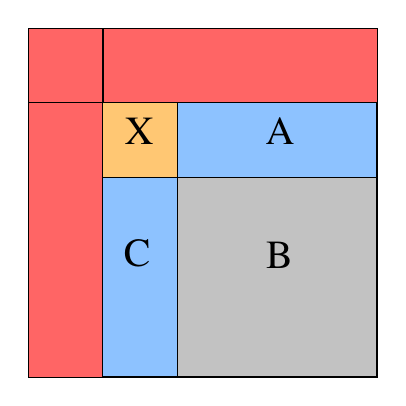
\begin{tikzpicture}[x=0.75pt,y=0.75pt,yscale=-1,xscale=1]
    %uncomment if require: \path (0,324); %set diagram left start at 0, and has height of 324
    
    %Shape: Square [id:dp5718523963116733] 
    \draw   (239,57) -- (407.28,57) -- (407.28,225.28) -- (239,225.28) -- cycle ;
    %Shape: Square [id:dp8609898911567822] 
    \draw  [fill={rgb, 255:red, 255; green, 101; blue, 101 }  ,fill opacity=1 ] (239,57) -- (274.97,57) -- (274.97,92.97) -- (239,92.97) -- cycle ;
    %Shape: Rectangle [id:dp1778431402239684] 
    \draw  [fill={rgb, 255:red, 255; green, 101; blue, 101 }  ,fill opacity=1 ] (275.12,57) -- (407.28,57) -- (407.28,92.8) -- (275.12,92.8) -- cycle ;
    %Shape: Rectangle [id:dp6200482171661257] 
    \draw  [fill={rgb, 255:red, 255; green, 101; blue, 101 }  ,fill opacity=1 ] (275.12,92.8) -- (275.12,225.11) -- (239,225.11) -- (239,92.8) -- cycle ;
    %Shape: Rectangle [id:dp5567096500887732] 
    \draw  [fill={rgb, 255:red, 141; green, 194; blue, 255 }  ,fill opacity=1 ] (311.09,128.94) -- (311.09,224.81) -- (274.97,224.81) -- (274.97,128.94) -- cycle ;
    %Shape: Square [id:dp7106049913134598] 
    \draw  [fill={rgb, 255:red, 255; green, 199; blue, 115 }  ,fill opacity=1 ] (274.97,92.97) -- (310.94,92.97) -- (310.94,128.94) -- (274.97,128.94) -- cycle ;
    %Shape: Rectangle [id:dp6402838940394686] 
    \draw  [fill={rgb, 255:red, 141; green, 194; blue, 255 }  ,fill opacity=1 ] (310.94,92.82) -- (406.81,92.82) -- (406.81,128.94) -- (310.94,128.94) -- cycle ;
    %Shape: Square [id:dp8611002911103105] 
    \draw  [fill={rgb, 255:red, 194; green, 194; blue, 194 }  ,fill opacity=1 ] (310.94,128.94) -- (407.02,128.94) -- (407.02,225.02) -- (310.94,225.02) -- cycle ;
    
    
    % Text Node
    \draw (284.31,98.68) node [anchor=north west][inner sep=0.75pt]  [font=\Large] [align=left] {X};
    % Text Node
    \draw (352.07,98.68) node [anchor=north west][inner sep=0.75pt]  [font=\Large] [align=left] {A};
    % Text Node
    \draw (283.81,157.77) node [anchor=north west][inner sep=0.75pt]  [font=\Large] [align=left] {C};
    % Text Node
    \draw (352.39,158.73) node [anchor=north west][inner sep=0.75pt]  [font=\Large] [align=left] {B};
    
    
    \end{tikzpicture}

\end{center}
The operation we are focused in is the following:
\[
    [C|B]-\frac{[C]}{X}\cdot [X|A]
\]

Visually, this can be seen as:

\begin{center}

    \tikzset{every picture/.style={line width=0.75pt}} %set default line width to 0.75pt        

    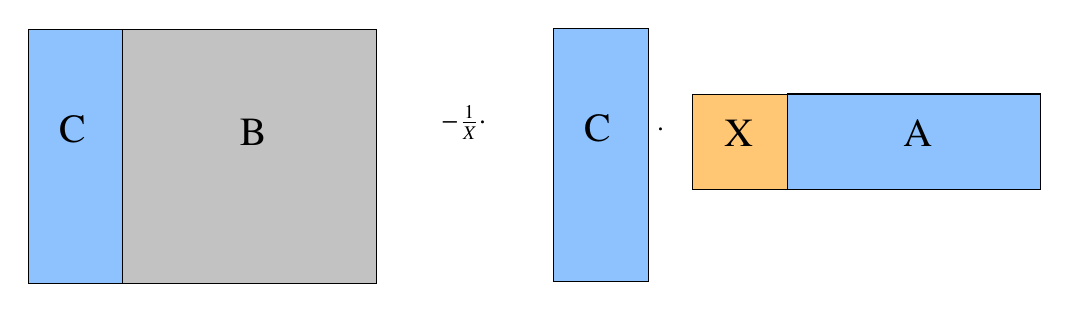
\begin{tikzpicture}[x=0.75pt,y=0.75pt,yscale=-1,xscale=1]
    %uncomment if require: \path (0,245); %set diagram left start at 0, and has height of 245
    
    %Shape: Rectangle [id:dp9607747510695368] 
    \draw  [fill={rgb, 255:red, 141; green, 194; blue, 255 }  ,fill opacity=1 ] (143.47,80.29) -- (143.47,202.32) -- (97.5,202.32) -- (97.5,80.29) -- cycle ;
    %Shape: Square [id:dp21312629022980478] 
    \draw  [fill={rgb, 255:red, 194; green, 194; blue, 194 }  ,fill opacity=1 ] (143.01,80.29) -- (265.31,80.29) -- (265.31,202.59) -- (143.01,202.59) -- cycle ;
    %Shape: Rectangle [id:dp7300626917834647] 
    \draw  [fill={rgb, 255:red, 141; green, 194; blue, 255 }  ,fill opacity=1 ] (396.5,79.47) -- (396.5,201.5) -- (350.53,201.5) -- (350.53,79.47) -- cycle ;
    %Shape: Rectangle [id:dp23600064291235356] 
    \draw  [fill={rgb, 255:red, 255; green, 199; blue, 115 }  ,fill opacity=1 ] (417.56,111.35) -- (463.34,111.35) -- (463.34,157.13) -- (417.56,157.13) -- cycle ;
    %Shape: Rectangle [id:dp0803219872663885] 
    \draw  [fill={rgb, 255:red, 141; green, 194; blue, 255 }  ,fill opacity=1 ] (463.34,111.16) -- (585.38,111.16) -- (585.38,157.13) -- (463.34,157.13) -- cycle ;
    
    % Text Node
    \draw (111.07,120.53) node [anchor=north west][inner sep=0.75pt]  [font=\Large] [align=left] {C};
    % Text Node
    \draw (198.23,121.76) node [anchor=north west][inner sep=0.75pt]  [font=\Large] [align=left] {B};
    % Text Node
    \draw (364.1,119.71) node [anchor=north west][inner sep=0.75pt]  [font=\Large] [align=left] {C};
    % Text Node
    \draw (431.64,122.17) node [anchor=north west][inner sep=0.75pt]  [font=\Large] [align=left] {X};
    % Text Node
    \draw (517.89,122.17) node [anchor=north west][inner sep=0.75pt]  [font=\Large] [align=left] {A};
    % Text Node
    \draw (295.46,115.55) node [anchor=north west][inner sep=0.75pt]    {$-\frac{1}{X} \cdot $};
    % Text Node
    \draw (399.21,126.24) node [anchor=north west][inner sep=0.75pt]    {$\cdot $};
    
    
    \end{tikzpicture}
    
\end{center}
The main problem with this operation is within how Python's Numpy interprets the matrices $[C]$ and $[X|A]$. It interprets it as a vector, not as a column/row matrix. This is a problem because the operation for multipliying matrices and vectors are different.

In order to solve the problem we have multiple options to choose from:


\begin{enumerate}
    \item By Submatrices Syntax
    
    The first option is to use the submatrices syntax, which can be summirized as taking a submatrix of a matrix using numpy syntax, doing so it will preserve the form of the matrix and not as a vector.

    \begin{lstlisting}[language=Python]
A[col + 1 :, col] = A[col + 1 :, col] / pivot
A[col + 1 :, col + 1 :] -= A[col + 1 :, :][:, [col]] @ A[[col], :][:, col + 1 :]
    \end{lstlisting}

    Note: The `@' symbol is the matrix multiplication operation in numpy.
    \item By New Axis Syntax
    
    The second option is to use the new axis syntax, which can be summirized as tacking directly the vector and making numpy to add a new axis to it, this way we transform the vector into a matrix and we can use the matrix multiplication operation.
    
    \begin{lstlisting}[language=Python]
A[col + 1 :, col] = A[col + 1 :, col] / pivot
A[col + 1 :, col + 1 :] -= A[col + 1 :, col][:, np.newaxis] @ A[col, col + 1 :][np.newaxis, :]
    \end{lstlisting}


    Note: The `@' symbol is the matrix multiplication operation in numpy.
    \item By using the Outer Product
    
    The outer product is a matrix operation that takes two vectors and returns a matrix, this operation is the same as the new axis syntax but it is more explicit and easier to understand.


    \begin{lstlisting}[language=Python]
A[col + 1 :, col] = A[col + 1 :, col] / pivot
A[col + 1 :, col + 1 :] -= np.outer(A[col + 1 :, col], A[col, col + 1 :])
    \end{lstlisting}

    \item Using a for loop
    
    The last option is to use a for loop to iterate over the rows and columns of the matrix, this way we can avoid the problem of the vector interpretation and we can use the normal multiplication operation of elements. This option is by far the first one that comes to mind and the most intuitive one, generally speaking.

    \begin{lstlisting}[language=Python]
for row in range(col + 1, n):
    A[row, col] = A[row, col] / A[col, col]  # Calculate the multiplier and store in A for later use
    A[row, col + 1 :] -= A[row, col] * A[col, col + 1 :]  # Update the remaining elements in the row using the multiplier
    \end{lstlisting} 
\end{enumerate}

To test these methods we will proceed by creating 100 random matrices for the sizes [500, 1000, 1500, 2000, 2500, 3000, 3500, 4000] and measure the length of time it takes for the algorithm to calculate the LU factorisation for each method. Note that all methods have exactly the same syntax before and after the options we have; therefore, we reduce possible noise.
\paragraph{Results}
The results of the mean of those 100 iterations for each size in seconds are as follows. 
\begin{table}[H]
    \centering
    \begin{tabular}{|l|l|l|l|l|l|}
    \hline
        \textbf{Matrix Size} & \textbf{Submatrices} & \textbf{New Axis} & \textbf{Outer Product} & \textbf{Loop} & \textbf{scipy} \\ \hline
        500 & 0.41335 & 0.169461 & 0.117083 & 0.465405 & 0.018257 \\ \hline
        1000 & 2.563606 & 1.522018 & 1.110119 & 2.176568 & 0.03057 \\ \hline
        1500 & 8.535015 & 5.212411 & 3.8087 & 5.579113 & 0.069611 \\ \hline
        2000 & 20.30588 & 12.333257 & 9.134406 & 10.942175 & 0.132066 \\ \hline
        2500 & 39.145535 & 23.998247 & 17.653031 & 19.098659 & 0.216267 \\ \hline
        3000 & 68.789119 & 41.919219 & 31.590708 & 29.468995 & 0.42402 \\ \hline
        3500 & 106.423081 & 64.700578 & 47.661064 & 42.445734 & 0.447992 \\ \hline
        4000 & 157.028937 & 96.519873 & 70.584879 & 58.448117 & 0.603978 \\ \hline
    \end{tabular}
    \caption{LU Methods Data in seconds}
\end{table}

On a visual plot:

\begin{figure}[H]
  \centering
    \includegraphics[scale=0.75]{Include/Images/Thesis/Analysis of Solutions/Linear Systems/LU Timings.png}
    \caption{LU Methods timings comparison}
    \label{fig:LU Methods comparison}
\end{figure}
\begin{figure}[H]
    \centering
    \includegraphics[scale=0.75]{Include/Images/Thesis/Analysis of Solutions/Linear Systems/LU Timings LOG.png}
    \caption{Log plot of LU methods timings}
    \label{fig:Log plot of LU methods}
\end{figure}

As we can observe from the tabular data and the plot, Scipy's method is by far the fastest, that is, due to the implementation using LAPACK's library~\cite{lapack99} which is compiled amongst other things, and the slowest is using the Submatrices syntax; surprisingly, the syntax using a for-loop improves over the other implementations as size increases, therefore even though this works for large sizes, using a for-loop that implements the reduction is the best choice overall the other methods (without accounting for Scipy's) since it is more readable and easier to understand, which is a key aspect in this work since we are trying to make the code as readable as possible for pupils.

For mere due diligence, we have calculate the slopes using  linear regression.
\begin{table}[H]
    \centering
    \begin{tabular}{|l|l|l|l|l|l|}
    \hline
        \textbf{} & \textbf{Submatrices} & \textbf{New Axis} & \textbf{Outer Product} & \textbf{Loop} & \textbf{scipy} \\ \hline
        slope & 2.885234 & 3.043451 & 3.071779 & 2.334054 & 1.813654 \\ \hline
    \end{tabular}
    \caption{LU Data slopes of Linear Regression}
\end{table}
In this last table, we can see that although the submatrices syntax was the slowest in the previous plots, is better than using the New Axis syntax, it must be noted that this will only be seen when the size of the matrix is humongous, and barely reachable in a sort span of time. 

\subsubsection{Examples}
	\input{Content/Thesis/Documentation/Examples/Linear Systems/LU Examples}


\subsection{Forward and Backward Substitution}
Undoubtedly, one of the key steps in solving a linear system is substitution, where we find the actual solutions to our system, that is why there exists two main numerical methods that are use, which are Forward and Backward substitution. These methods take a triangular matrix (lower and upper, respectively) and make the necessary substitutions.

The first approach, forward substitution, substitutes the first row and then moves "forward" in the next variables using the already computed values. Backward substitution is analogous, but instead of starting with the first variable, it starts with the last (since this method takes an upper triangular matrix) and moves backwards until it has reached the first variable.

The reason of implementing this method is that we want BNumMet to be self-contained, that is, we want to have all the necessary tools to solve a linear system without the need of external libraries.

The algorithms were based upon Fernando Terán de Vergara's course notes for the Master in Applied \& Computational Mathematics~\cite{Vergara}.
\subsubsection{Examples}
\textbf{Forward Substitution}
	\input{Content/Thesis/Documentation/Examples/Linear Systems/Forward Substitution Examples}
 \textbf{Backward Substitution}
	\input{Content/Thesis/Documentation/Examples/Linear Systems/Backward Substitution Examples}
\subsection{QR Decomposition}
Alongside the LU decomposition, there exists another decomposition known as the QR Decomposition, similarly to the LU decomposition, the concept behind QR is decompose a matrix into a product of two, in this case, it will be a product of an orthogonal matrix (Q) and an upper triangular matrix(R). We have implemented this technique using Householder reflectors which is the fundamental method to implement this decomposition.

The reason of implementing these method as a standalone is to give an additional feature to BNumMet and also to the students. %Though a QR solver is used to solve the Least Squares problem, these method as an autonomous is not used, only an optimized variant for the solver which takes into consideration the independent terms.

The algorithm was based upon Fernando Terán de Vergara's course notes for the Master in Applied \& Computational Mathematics~\cite{Vergara}.
\subsubsection{Examples}
\input{Content/Thesis/Documentation/Examples/Linear Systems/QR Decomposition Examples}

\subsection{LU Solver}
We implemented the function that solves a linear system $Ax=b$ using the LU factorization and forward and backward substitution as part of the Linear Systems Package. The reason for implementing these is to add extra features to BNumMet as well as give the student a written version of the solver, as it is trivial to implement once you have the aforementioned methods. Apart from appropriately commenting the code, no other considerations have been made.
\subsubsection{Examples}
	\input{Content/Thesis/Documentation/Examples/Linear Systems/LU Solver Examples}

\subsection{QR Solver}
Similarly to the LU Solver, we have added a functionality that will be critical on solving the Least Squares Problem, that is the QR solver. The reason for the QR solver, aside from being used in the Least Squares Problem to avoid the ill-conditioning of solving the Least Squares Problem using the well-known formula of $A^T A x= A^T b$, is that it implements an optimized version of QR taking into account the fact that we are solving a Linear System, in this optimized version, the algorithm does not compute the Q matrix but rather it applies it to the independent terms wihtout storing such matrix and then uses the backward substitution on R (which is computed).

Not only does this method provides students with another approach on solving linear systems or the Least Squares Problem, but it also grants the underlying procedure of the well-known Matlab Backslash.

The algorithm is based upon C.Moller's~\cite{doi:10.1137/1.9780898717952} and Fernando Terán's work~\cite{Vergara}
\subsubsection{Examples}
\input{Content/Thesis/Documentation/Examples/Linear Systems/QR Solver Examples}



\section{Interpolation}
Undoubtedly, one of the pinnacles of numerical methods is trying to find a function that passes through a fixed set of points, in hopes of understading how the this points are related to each other, all this using what is known as an `Interpolating Function' which is a function that passes through all the points of a given set. Many different functions exists for a given set of points, in this package, we have built some of the various methods for interpolating a function; however, despite the simplicity of the method's implementation, a general analysis has been conducted on a specific method of implementing the function evaluation; this analysis will be presented after a brief description of the methods.

The following algorithm implementations that we have realized will be detailed in this section:
\begin{itemize}
    \item Polinomial Interpolation \algoref{alg:Polinomial Interpolation}
    \item Piecewise Linear Interpolation \algoref{alg:Piecewise Linear Interpolation}
    \item Piecewise Cubic Hermite Interpolation \algoref{alg:Piecewise Cubic Hermite Interpolation}
    \item Piecewise Cubic Interpolatory Splines \algoref{alg:Piecewise cubic Interpolatory Splines}
\end{itemize}

All of the algoritmhs have three main parameters, 
\begin{itemize}
    \item \textbf{X}: The x-coordinates of the points we want to interpolate.
    \item \textbf{Y}: The y-coordinates of the points we want to interpolate.
    \item \textbf{U}: The x-coordinates of the points we want to evaluate. This is what we call the mesh.
\end{itemize}
And all of them return the y-coordinates of the points we want to evaluate.

Some of the above algorithms were based uppon C. Moller's reference~\cite{doi:10.1137/1.9780898717952}.

\subsection{Polynomial Interpolation}
This approach performs a polynomial interpolation of a given collection of points; it is one of the fundamental ways of interpolation and the root in the solutions of many error estimation problems. 

The main goal of this interpolation is to find create a polynomial of degree $n-1$ (being $n$ the number of points) that passes through all the points of the set. The algorithm implemented uses the Lagrange interpolation formula~\cite{mathworldLagrange}.
\subsubsection{Examples}
	\input{Content/Thesis/Documentation/Examples/Interpolation/Polinomial Interpolation Examples}


\subsection{Piecewise linear interpolation}
Following the polynomial interpolation approach, the next step is to extend this notion to piecewise functions; but firstly we will make an intial step using linear functions, that is, we will interpolate the points using a line that passes through two points, this is known as piecewise linear interpolation. 

The way the algorithms works is to find the closest two points from the the point of the mesh all within the given dataset, and the use the calculated slope in order to evaluate the point of the mesh.

\subsubsection{Examples}
	\input{Content/Thesis/Documentation/Examples/Interpolation/PieceWise Linear Interpolation Examples}

\subsection{Piecewise cubic interpolation}
Following the Piecewise Linear interpolation we are going to use the same idea but with a cubic function, that is, we will interpolate the points using a cubic function that passes through four points, this is known as piecewise cubic interpolation. 

This interpolating polynomial is twice continuously differentiable, and hence each piecewise function is a cubic spline, as well as, having the boundary conditions know as `not-a-knot'~\cite{doi:10.1137/1.9780898717952} which as Mathwork's states at the first and last interior break, the third derivative of the interpolating function is continuous (up to round-off error)~\cite{notAknot}.


\subsubsection{Examples}
\input{Content/Thesis/Documentation/Examples/Interpolation/Splines Examples}


\subsection{Piecewise Cubic Hermite interpolation}
To end this section, we will present a different approach to piecewise cubic interpolation, this time we will use the Piecewise Cubic Hermite Interpolation Polynomial (P.C.H.I.P.) which is a form of cubic spline interpolation that uses, as per the name indicates, cubic polynomials but whose slopes are explicitly given (in the case of this algorithm they are calcutated according to Mathworks implementation), in the algorithm this is done by looking at the sign of the slopes (using an approximation to the derivative) and then using the harmonic mean to calculate the slope of the interpolating polynomial, this works for the interior points, for the exterior ones . 

The `pchip' function is a Python implementation of the Piecewise Cubic Hermite Interpolation Polynomial (P.C.H.I.P.) based on an old Fortran program by Fritsch and Carlson~\cite{doi:10.1137/0717021}.

\subsubsection{Examples}
	\input{Content/Thesis/Documentation/Examples/Interpolation/PCHIP Examples}



\subsection{Interpolation implementation analysis}

Similar to the discussion in the linear systems package, we discovered numerous ways a student could implement one part of the method, this one part refers to the lines of code that evaluates the value ($f(x)$) of the points of the mesh. 

In short, for interpolating, one needs to compute the interpolating polynomial as well as evaluating it. The following piece of code is related with the evaluation of piecewise interpolation methods. Particularly, one needs to find in which subinterval a point of the mesh is in, all done to then properly evaluate the interpolating function of that point

The code section may be summarized as follows: 


\begin{algorithm}[H]
\SetAlgoLined
\For{$j \gets 1$ \KwTo $n-2$} {
$k[x_j <= u] \gets j$
}
$s \gets u - x_k$\\
$v \gets y_k + s * \Delta_k$

\caption{Extract from Interpolation's algorithm}
\end{algorithm}
As one can see, this portion of the code assign values to an array $k$ which is then used to access the index of the array $y$ and $x$, this is done in order to apply the specific formula to the approiate section of the mesh. But, we know for a fact that $k$ is an array and we cannot use it as index, per se, thus we need to find a way to access the index of the array $y$ and $x$ using the values of $k$.

Note: It should be noted that other algorithms may have different calculations, however for the sake of simplicity, we are generalizing the portion of code.



We might implement this section of code in a variety of ways, including:
\begin{enumerate}
    \item List Comprehension: Python offers a compact form for adding items to a list, in particular list comprehension, for a general reader a list comprehension is based on mathematical notation that is $\left\{ 3n\ | n\in \mathbb{N},\ 0\leq n\leq 25\right\}$ can be written in Python as \lstinline|[3*n for n in range(0,26)]|, generally speaking list comprehension is faster than classical loops~\cite{PythonSpeedPerformanceTips}, however, a better approach would be using functional maps which are cognitively more difficult to understand, thus not the purpose of this project.
    
    This is an approach that will iterate through the elements in $k$ and therefore we will be able to access the index of the array $y$ and $x$.

    \item Using NumPy's \textit{fancy} Indexing: Similarly to Matlab, NumPy offers a way to broadcast a list, that is we can access the items of a list using another list. This is an approach developed by NumPy that will iterate through the elements in $k$ in a sugar-coated syntax way. In itself, it is a list comprehension but with a different syntax and different internal mechanisms.
    
    Altough it is cognitively more complicated than list comprehensions; it is a syntax that is widely used in the numerical methods realm and might be a fair competitor over list comprehensions.
    
    
    
\end{enumerate}
\paragraph{Results}
To correctly test the implementations we will fix 6 interpolation pairs and then run 100 iterations for different meshes sizes with random values (to also check the ability to sort the mesh points), then after those 100 iterations are over, we will calculate the mean, the results are the following:
\begin{figure}[H]
    \centering
    \includegraphics[scale=0.9]{Include/Images/Thesis/Analysis of Solutions/Interpolation/Interpolation Timings.png}
    \caption{Interpolation Timings}
    \label{fig:Interpolation Timings}
\end{figure}

As we can visually observe, the use of List Comprehensions is by far the worst of the two, and should be discarded for this particular case. We can also see how much the \textit{fancy} indexing improves the overall speed.Applying linear regression on both sets of data we get the following results:
\begin{enumerate}
    \item \textbf{Linear Regression \textit{fancy} indexing}: \\
        $y = 3.4812\cdot10^{-08}x + 0.0002$ \\
        Slope: $3.48119\cdot10^{-08}$
    \item \textbf{Linear Regression List Compresion}: \\
        $y = 2.0237\cdot10^{-06}x + 0.0003$ \\
        Slope: $2.02374\cdot10^{-06}$
\end{enumerate}

Overall, not only does the choice of \textit{fancy} indexing is by far the fastest (around 2 orders of magnitude) but it also provides students a syntax that will be used during their learning of numerical methods, though it must be noted, the use of for-loops might be ideal for didactic purposes to teach students what could be behind the notation of this \textit{fancy} indexing.





\section{Non Linear Equation Solver Package}
As part of extending BNumMet's functionality, we decided to implement the numerical methods associated with solving nonlinear equations because it is a topic that, like the others, is widely taught in a numerical methods course and is a fundamental approach to solving most equations that may not be solvable using a linear approach.

The following algorithm implementations that we have realized will be detailed in this section:
\begin{itemize}
    \item Bisection method \algoref{alg:Bisection Method}
    \item Secant  method \algoref{alg:Secant method}
    \item Newton-Raphson \algoref{alg:Newton-Raphson Method}
    \item Inverse Quadratic Interpolation \algoref{alg:IQI Method}
    \item Brent-Dekker \algoref{alg:zBrentDekker} 
\end{itemize}

Except for the last method, all of the approaches are quite straightforward, with the main exception being that the input function may be multidimensional, but only the zero will be located in one of the dimensions. In addition, an iteration counter has been introduced for student study of the efficiency of the various methods.

\subsection{Bisection}
We have implemented the well known method of the bisection method, a method that at every iteration divides the search interval into two half's and takes the one whose sign at the extremes change. No extra considerations have been taken into account except for adding the appropriate comments for any student to know what every step is doing.

The algorithm is based upon Cleve's implementation \cite{doi:10.1137/1.9780898717952}.
\subsubsection{Examples}
	\input{Content/Thesis/Documentation/Examples/NonLinear/Bisection Examples}

\subsection{Newton's Method}
Most numerical methods classes use this approach to illustrate the secant method, which is why we built it; nevertheless, it should be noted that according to the method, this is the only one that needs the input of the derivative.
\subsubsection{Examples}
	\input{Content/Thesis/Documentation/Examples/NonLinear/Newtons Examples}


\subsection{Secant Method}
As a continuation of Newton's approach, it is critical to apply the Secant method, which generalizes Newton's method by approximating the derivative and eliminating the necessity for the derivative that Newton's method requires. 

The algorithm is based upon Cleve's implementation \cite{doi:10.1137/1.9780898717952}.
\subsubsection{Examples}
	\input{Content/Thesis/Documentation/Examples/NonLinear/Secant Examples}

\subsection{Inverse Quadratic Interpolation (I.Q.I.)}
The aim is to utilize quadratic interpolation to approximate the inverse of f, and further iterations will result in the zero we want. It should be noted that this method is often used as part of another method that we will examine later \cite{10.5555/2553197}, that is why we created it as a standalone to offer students with a glimpse of what the method is about without additional code that may interfere with the learning process.

The algorithm is primarily based upon \cite{kreyszig11}  as well as Moller's implementation \cite{doi:10.1137/1.9780898717952}.
\subsubsection{Examples}
	\input{Content/Thesis/Documentation/Examples/NonLinear/IQI Examples}


\subsection{Brent-Dekker's Algorithm}
Brent Dekkers algorithm is one of the methods that combines the previously discussed methods into a method that will improve the number of evaluations a specific method may require while also eliminating some of the caveats that, for example, the secant method has, where there are functions where this latter method does not converge.  It should be noted that this approach was first developed by Dekker, Wiengarten, and their colleagues, only to be modified by Brent to improve convergence. \cite{brent2002algorithms} 

The fundamental idea of Brent-Dekker's Algorithm is to apply the bisection, secant, and if possible the I.Q.I. method, the fundamental criteria of choice is firstly the availability of the application of I.Q.I. which requires three distinct points, after checking that, if it applies I.Q.I is saved, otherwise the secant is saved to then be compared with the bisection algorithm, whichever of the two passes a tolerance criteria given then they will be applied and the next iteration will commence.


In BNumMet, we used Brent's original approach \cite{Press2007} which has a Fortran implementation of the algorithm. The use of this work rather than Matlab's was for a variety of reasons, one of them is the license under which Matlab allows the code to be used; since our goal was to follow open source initiatives, we needed to use the original one. We also wanted to show students the historical accuracy of the algorithm and present a method that preserves the historical context as well as its current properties. 

In the next paragraph, we will examine the several implementations we discovered, including Matlab's implementation, the original implementation, and Scipy's implementation.

\subsubsection{Analysis of implementations}
The analysis of this package differs from the previous two (linear systems and interpolation packages), where we draw our attention to the syntax and it benefits, in this analysis we will focus on comparing the same method over different plausible implementations that might differ slightly on the code but have a humongous impact on the results of such slight algorithmic differences.

In particular, we will focus on the different implementations the Brentt-Dekker algorithm can have; we will tackle the following:
\begin{enumerate}
    \item Scipy's Brentt Method: The commonly used library for scientific computing has its own implementation of Brent-Dekker's Algorithm. However, the code is not publicly visible. We will discuss how to obtain results without knowing how it works.
    \item Matlab's - Cleve Moller' Implementation: As we discussed, this project has the underlying idea of Cleve Moller's book \cite{doi:10.1137/1.9780898717952}, that is why we have made the translation of this algorithm into Python to properly test it, though it must be noted we will not be using it in our package as a standalone, since we do not own the right to do so.
    \item Original Brent-Dekker's Algorithm: Following the original documentation of Brent \cite{brent2002algorithms} we have translated the procedure given in Chapter 4 of Brent's work into Python.
\end{enumerate}

In this analysis we are interested in how many function evaluation does the algorithm need to find the root, the fundamental reason that we are interested in the number of evaluations is because this types of algorithms do not have an excessive algorithmic complexity, making the evaluation of the function that (most likely) will be nonlinear carry all the computational cost, that is why we need to find the number of evaluations. However, we are unable to look at Scipy's code to tamper with it to obtain our desired result, to properly proceed I want to digress from the discussion at hand and focus on how we can find the number of function evaluations without the need of having the actual implementation.

\paragraph{Finding function evaluations without external code} As a thought experiment, imagine you have a machine that is protected so as not to be opened or tampered with, this machine can only take in a function $f(x)$ and outputs its zero (for arguments sake, suppose it can be done without any problems), this machine does not output how many times did it use the function to calculate or has a small light that shows how it is processing. We can only input functions and have as an output the location of the zero. 




\tikzset{every picture/.style={line width=0.75pt}} %set default line width to 0.75pt        

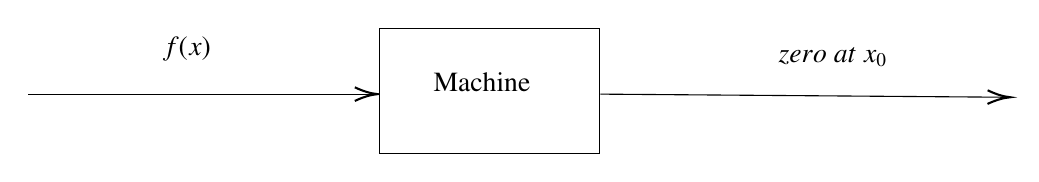
\begin{tikzpicture}[x=0.75pt,y=0.75pt,yscale=-1,xscale=1]
%uncomment if require: \path (0,141); %set diagram left start at 0, and has height of 141

%Straight Lines [id:da07216189034981646] 
\draw    (95,71.28) -- (261.29,71.28) ;
\draw [shift={(263.29,71.28)}, rotate = 180] [color={rgb, 255:red, 0; green, 0; blue, 0 }  ][line width=0.75]    (10.93,-3.29) .. controls (6.95,-1.4) and (3.31,-0.3) .. (0,0) .. controls (3.31,0.3) and (6.95,1.4) .. (10.93,3.29)   ;
%Shape: Rectangle [id:dp6037570291001613] 
\draw  [fill={rgb, 255:red, 255; green, 255; blue, 255 }  ,fill opacity=1 ] (264.3,39.53) -- (370.12,39.53) -- (370.12,100) -- (264.3,100) -- cycle ;
%Straight Lines [id:da284111323999086] 
\draw    (370.62,71.28) -- (566.14,72.78) ;
\draw [shift={(568.14,72.79)}, rotate = 180.44] [color={rgb, 255:red, 0; green, 0; blue, 0 }  ][line width=0.75]    (10.93,-3.29) .. controls (6.95,-1.4) and (3.31,-0.3) .. (0,0) .. controls (3.31,0.3) and (6.95,1.4) .. (10.93,3.29)   ;

% Text Node
\draw (158.6,42.52) node [anchor=north west][inner sep=0.75pt]    {$f( x)$};
% Text Node
\draw (455.28,47.56) node [anchor=north west][inner sep=0.75pt]    {$zero\ at\ x_{0}$};
% Text Node
\draw (289,59.67) node [anchor=north west][inner sep=0.75pt]   [align=left] {Machine};


\end{tikzpicture}



One could argue why not create a function that counts the evaluation every time it is invoked; something of this sort will reassemble: 
\begin{lstlisting}
FUNCTION 
    IN : x
    PERFORM : 
        evaluations +=1
    OUT : f(x)
\end{lstlisting}

But most programming languages lack the ability to auto-initialise the value, and even if initialised it must be done inside the function itself which will be reset every function evaluation.

Imagine we can create a function (think of if as a piece of hardware) that can safely be input to our machine and still have our expected zero, but we  can create one 'invisible' cable that is connected to a light outside the machine, and every time it evaluates the function, the light is turned on (or in this case a counter is updated). To do such thing, we must draw our attention to Global Variables, variables that are within the reach of the entire execution of a program and can be edited and accessed anywhere in the code. 

This idea will look like 
\begin{lstlisting}
global evaluations = 0
FUNCTION 
    IN : x
    PERFORM : 
        evaluations +=1
    OUT : f(x)
\end{lstlisting}


Once this link is created, we only need to reset the counter every time we input a new function, and we will obtain the evaluations they did of the function.



\tikzset{every picture/.style={line width=0.75pt}} %set default line width to 0.75pt        

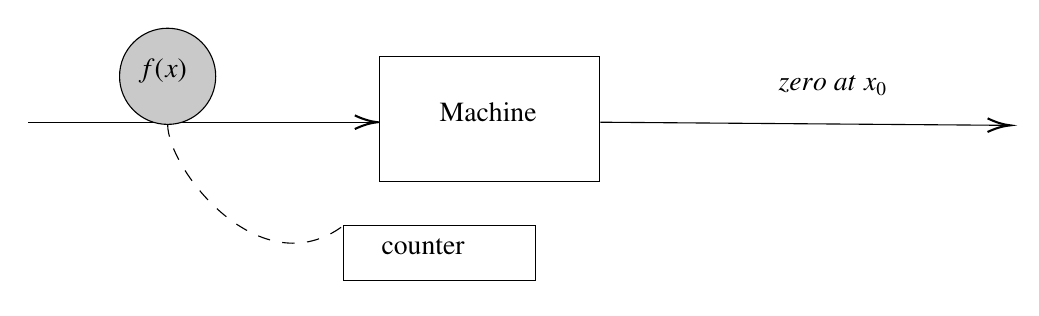
\begin{tikzpicture}[x=0.75pt,y=0.75pt,yscale=-1,xscale=1]
%uncomment if require: \path (0,190); %set diagram left start at 0, and has height of 190

%Straight Lines [id:da8004978280594872] 
\draw    (99,89.28) -- (265.29,89.28) ;
\draw [shift={(267.29,89.28)}, rotate = 180] [color={rgb, 255:red, 0; green, 0; blue, 0 }  ][line width=0.75]    (10.93,-3.29) .. controls (6.95,-1.4) and (3.31,-0.3) .. (0,0) .. controls (3.31,0.3) and (6.95,1.4) .. (10.93,3.29)   ;
%Shape: Rectangle [id:dp04043727048803203] 
\draw  [fill={rgb, 255:red, 255; green, 255; blue, 255 }  ,fill opacity=1 ] (268.3,57.53) -- (374.12,57.53) -- (374.12,118) -- (268.3,118) -- cycle ;
%Straight Lines [id:da458025777694687] 
\draw    (374.62,89.28) -- (570.14,90.78) ;
\draw [shift={(572.14,90.79)}, rotate = 180.44] [color={rgb, 255:red, 0; green, 0; blue, 0 }  ][line width=0.75]    (10.93,-3.29) .. controls (6.95,-1.4) and (3.31,-0.3) .. (0,0) .. controls (3.31,0.3) and (6.95,1.4) .. (10.93,3.29)   ;
%Flowchart: Connector [id:dp3688737316817359] 
\draw  [fill={rgb, 255:red, 201; green, 201; blue, 201 }  ,fill opacity=1 ] (143,67.17) .. controls (143,54.37) and (153.37,44) .. (166.17,44) .. controls (178.96,44) and (189.33,54.37) .. (189.33,67.17) .. controls (189.33,79.96) and (178.96,90.33) .. (166.17,90.33) .. controls (153.37,90.33) and (143,79.96) .. (143,67.17) -- cycle ;
%Curve Lines [id:da6747445781275441] 
\draw  [dash pattern={on 4.5pt off 4.5pt}]  (166.17,90.33) .. controls (166.33,112.33) and (211,169) .. (251,139) ;
%Shape: Rectangle [id:dp15460904797277109] 
\draw  [fill={rgb, 255:red, 255; green, 255; blue, 255 }  ,fill opacity=1 ] (251,139) -- (343.33,139) -- (343.33,165.33) -- (251,165.33) -- cycle ;

% Text Node
\draw (459.28,65.56) node [anchor=north west][inner sep=0.75pt]    {$zero\ at\ x_{0}$};
% Text Node
\draw (151,57.4) node [anchor=north west][inner sep=0.75pt]    {$f( x)$};
% Text Node
\draw (268,144) node [anchor=north west][inner sep=0.75pt]   [align=left] {counter};
% Text Node
\draw (296,78.67) node [anchor=north west][inner sep=0.75pt]   [align=left] {Machine};

\end{tikzpicture}

\paragraph{Results}
To test it we will implement the thought experiment in code and proceed in the following manner, we will create a function $f(x) = (x-a)\cdot x^{i}$, where $a$ will be either $1$ or $0.1$, a number that can be written in floating-point expression and one that cannot, the $i$ will be the exponent of the function which will take odd values. We will run the 3 aforementioned methods once (since in this case the algorithms are purely deterministic, as they do not rely on time) for different interval widths starting at $0.8$ and ending in $1.1+j$ where j will be increasing from 1 to 10000 in step sizes of 1. Using in all the methods the same input tolerance.

Our goal with this test will be firstly to prove the effectiveness of the original algorithm and the implementation in python with respect to the other two, as well as, observing if we have an algorithmic advantage or not with these aforementioned methods.

We will then take the number of evaluations and the value of x at where the zero is found in order to measure the relative error. The plots will not be in the whole range of step sizes but a smaller sample size of 75 step sizes

\subparagraph{For $a=1$}
As we can observe in the first plot of\imgref{fig:NonLinear 3 method Results for a=1 same tolerance} Scipy's implementation of Brent-Dekker's Algorithm is the worst in term of number of evaluations, and Matlab's has almost everywhere a similar behaviour in number of evaluations. Looking at the second plot, we see that even though BNumMet's implementation was better in terms of evaluations, it is the worst in terms of relative error, and Matlab's is similar to Scipy's but slightly worst.

One question rises from here: will BNumMets implementation improve - in terms of having a lower number of function evaluations - if we reduce the tolerance, at the risk of number of evaluations - but as seen, we still have room for tweaking. In fact, we can improve the relative error of BNumMets by decreasing the tolerance and still have an advantage over Scipy's implementation almost everywhere \imgref{fig:NonLinear 3 method Results for a=1 BNumMet smaller tolerance}

This results proves that the original implementation of Brent-Dekker is better than Scipy's, because at a lower number of function evaluations we achieve a better relative error. 

\subparagraph{For $a=0.1$}
The same discussion of $a=1$ remains valid to the case $a=0.1$, it must be noted that in this case the plots show a extravagant behaviour, with the number of evaluations, at certain points, the evaluations remain the same regardless of the interval size. On the first plot \imgref{fig:NonLinear 3 method Results for a=0.1 same tolerance} we observe that BNumMet takes the leading position while on the second plot, there remains a high relative error but closer to Matlab's on the overall scheme.

Incrementing the input tolerance to BNumMet's implementation, we observe \imgref{fig:NonLinear 3 method Results for a=0.1 BNumMet smaller tolerance} that not only does BNumMet's implementation offer a lower number of function evaluations but also it provides a better relative error in comparison to Scipy's implementation.

All in all, the decision to implement the original Brent-Dekker was a good choice; not only does it preserve the historical algorithm but also improves on the well-known library of Scipy.

\begin{sidewaysfigure}[H]
    \centering
    \includegraphics[width=\textwidth]{Include/Images/Thesis/Analysis of Solutions/NonLinear AS/NonLinear 3 method Results a-1.png}
    \caption{NonLinear 3 method Results for $a=1$ same tolerance}
    \label{fig:NonLinear 3 method Results for a=1 same tolerance}
\end{sidewaysfigure}

\begin{sidewaysfigure}[H]
    \centering
    \includegraphics[width=\textwidth]{Include/Images/Thesis/Analysis of Solutions/NonLinear AS/NonLinear 3 method Results Small Tol Bnum a-1.png}
    \caption{NonLinear 3 method Results for $a=1$ BNumMet smaller tolerance}
    \label{fig:NonLinear 3 method Results for a=1 BNumMet smaller tolerance}
\end{sidewaysfigure}

\begin{sidewaysfigure}[H]
    \centering
    \includegraphics[width=\textwidth]{Include/Images/Thesis/Analysis of Solutions/NonLinear AS/NonLinear 3 method Results a-0.1.png}
    \caption{NonLinear 3 method Results for $a=0.1$ same tolerance}
    \label{fig:NonLinear 3 method Results for a=0.1 same tolerance}
\end{sidewaysfigure}

\begin{sidewaysfigure}[H]
    \centering
    \includegraphics[width=\textwidth]{Include/Images/Thesis/Analysis of Solutions/NonLinear AS/NonLinear 3 method Results Small Tol Bnum a-0.1.png}
    \caption{NonLinear 3 method Results for $a=0.1$ BNumMet smaller tolerance}
    \label{fig:NonLinear 3 method Results for a=0.1 BNumMet smaller tolerance}
\end{sidewaysfigure}


\subsubsection{Examples}
	\input{Content/Thesis/Documentation/Examples/NonLinear/Brent Dekker Examples}

\section{Random Number Generator Package}
To expand the techniques available in BNumMet even further, we will incorporate a lesser-known field of numerical methods, namely the implementation of generators for (pseudo) random numbers. The underlying motivation for its development is our interest about how random number generators function, as well as allowing the end-user to study a side of numerical techniques that is not generally taught. We should also mention that this package was not originally intended to be developed, but due to some extra time, we decided it would be beneficial to include it.

Many of the suggested techniques rely on specific values being initialized, so we used a Python dictionary to help students understand the meaning of each variable by associating a key with its value; this dictionary is then used as a global dictionary in the appropriate method.

In this section the following algorithms had been implemented by the author of this work:
\begin{itemize}
    \item Lehmers Random Number Generator \algoref{alg:lehmersrand}
    \item Marsaglia Random Number Generator \algoref{alg:Marsaglia Random Number Generator Algorithm}
    \item Mersenne Twister Random Number Generator \algoref{alg:Mersenne Twister Random Number Generator}
\end{itemize}

\subsection{Lehmer's Generator}
Lehmer's Random Number Generator is one of the simplest yet most elegant generators available. This type of generator is a Linear Congruential generator, which is defined by the following recurrence relation~\cite{payne1969coding,park1988random}.
\[x_{n+1} = k\cdot x_n \mod{n}\]

In the case of Lehmer's generator it follows:
\[x_{n+1} = (a\cdot x_n+c) \mod{n}\]
The selection of $a,c,n$ and $x_0$ is critical, and some values have been proposed for optimal generation; one of these values has been used as the method's default initializer, in particular:
\[a= 7^5, c=0, m=2^{31}-1, x_0 = 1 \]

These values ensure that this generator works properly, but some bad generators can be found, which is an interesting exercise for the student to search for or come up with. Additionally it is worth mentioning that the developped function allows for input parameters to be set.

The algorithm implementation was based upon Moller's work~\cite{doi:10.1137/1.9780898717952}.
\subsubsection{Examples}
	\input{Content/Thesis/Documentation/Examples/Random/Lehmers Examples}


\subsection{Marsaglia's Generator}

In the original paper~\cite{10.1214/aoap/1177005878} Marsaglia expands on random number generators by providing a generator that is born from a type of relation such as Fibonacci, those generators that add or subtract previous values from the current value, but in Marsaglia's case this generator has some \textit{lag} added to it, that is it extends the appearance of the value that would be expected without \textit{lag}. It is accomplished by introducing two parameters know as $lag_s$ and $lag_r$ as well as a $carry$ variable which will be $1$ if the generated number is negative - to which the $base$ will be added - and $0$ if the generator produced a positive number. This $carry$ variable is what gives the name to this type of generator which are known as $add-with-carry$ or $subtract-with-borrow$

One of the complexities of this method is that it generates primarily integer numbers and is limited to the base it accepts as input; however, dividing by the base (the largest number in the generator) produces a decimal number between 0 and 1. Some input arguments were proposed, but as we saw in Lehmer's generator, some default parameters were provided. 
\[base = 2^{31}-1, lag_r=19, lag_s=7, carry=1, seed\_tuple = (1,1)\]
This set of values was proposed in the original paper; it is also worth noting that we used the subtract with borrow method, despite the fact that the addition with carry method is analogous. We strongly encourage students to try to find ill-inputs that generate patterns in their output.

We have implemented the algorithm using the original approach of Marsaglia~\cite{10.1214/aoap/1177005878}.
\subsubsection{Examples}
	\input{Content/Thesis/Documentation/Examples/Random/Marsaglias Examples}


\subsection{Mersenne Twister Generator}
The Mersenne Twister is an algorithm first introduced by Makoto Matsumoto and Takuji Nishimura~\cite{matsumoto1998mersenne}. According to the creators, the choice of parameters may produce a period (repetitions of random numbers) of $2^{19937}-1$ while only requiring 624 words of memory and every word is made up of 32 bits - on the original implementation, newer ones exists with 64 bits. Most notably, it is the most often used generator, serving as the default generator for the Python and R programming languages.

We opted to implement the technique due to its popularity, even if the mathematics behind it are outside the scope of this project. We reckon the code is simple and does not require a lot of focus to comprehend what it is doing. Furthermore, we wanted to give students with commonly utilized approaches, and the Mersenne Twister is unquestionably one of them.

As Makoto and Takuji did, they ran a battery of tests to prove the generation of random numbers; similarly, we will assess the efficacy of this method.

The implementation of the method was based upon the original work~\cite{matsumoto1998mersenne} which contains a C implementation.
\subsubsection{Analysis of solution}
One question that arises in Random Number Generators is, how can we make sure our generator is actually random?, in this section we will dive into how we have tested our Mersenne Twister function.

The reference we have followed is~\cite{smid2010statistical}, which develops a suite of tests to check different random number generators, and we have used an already developed version of this suite for Python~\cite{InsaneMonster2022}, since it was out of the scope of this project. 

Some discussion of the test we are eligible to test are the following.


\begin{enumerate}
\item  \textbf{Monobit test}: This test purpose is to count how many zeros are there in the sequence, if it is close (up to some epsilon) to ½ then the tests will pass. This is a crucial test inside the suite since if this test fails, the rest will not pass.

\item  \textbf{Frequency within a Block: }The test is analogous to the Monobit but instead of counting number of zeros in the entire string, it counts the frequency of 1 appearing in M-sized blocks, it should be close to M/2 plus or minus epsilon. 

\item  \textbf{Runs Tests: }This test counts the number of runs the sequence has. A run of length \textit{k} consists of exactly \textit{k} identical bits and is bounded by a bit of opposite value. 

\begin{enumerate}
\item  ``01111110'' : Run of length 6
\end{enumerate}


If the lengths are the ones one could expect from a random number, then the test will pass.


\item  \textbf{Longer Runs Test}: In this case, the goal is to determine if the longest run length of ones is consistent with what one can expect from a random number.  An irregularity in the length of ones, implies an irregularity in the length of zeros.

\item  \textbf{Discrete Fourier Spectral Test}: It tries to detect periodic features of the run, it applies the Discrete Fourier Transform and count the peaks, the main goal is to find if the peaks that exceed the 95\% threshold are less than 5\%.

\item  \textbf{Non-overlapping Template Matching:} The test tries to find generators that produce many occurrences of a aperiodic pattern, it searches on blocks of m bits for these types of patterns.

\item \textbf{ Serial test}: This test focuses on determining the number of occurrences of the $2^m$ length of bit patterns and checking if they are one that is to be expected, since random sequences have uniformity, so each sequence has the same probability of appearing. Were we to take $m=1$ we would have the same results as in the monobit test.

\item  \textbf{Approximate Entropy Test: }This is exactly the serial test, but compares with 2 consecutive blocks of lengths $m$ and $m+1$.

\item \textbf{ Cumulative sums: }This test tries to find which is the maximal length of a random walk, assuming a $0\ =\ -1$ and summing all the sequence, it should be close to zero.

\item \textbf{ Random Excursion: }It checks that the number of cycles that have k visits in a cumulative sum walk is that of a properly random test.

\begin{enumerate}
\item A cycle consists of a sequence of steps taken at random that begin at and return to the origin.
\end{enumerate}

\item \textbf{ Random Excursions Variant Test: }Counts how many times a particular state is visited in a random cumulative sum.
\end{enumerate}

\paragraph{Results}
To test it we will generate a total of 100 random integer numbers and run the battery of test through that sequence.
\begin{lstlisting}[language=Python]
import numpy
from nistrng import *

clear_mt_vars()
# Test genrand from nistrng
sequence = numpy.array([genrand() * 0xFFFFFFFF for i in range(100)], dtype=numpy.uint64)


binary_sequence: numpy.ndarray = pack_sequence(sequence)

# Check the eligibility of the test and generate an eligible battery from the default NIST-sp800-22r1a battery
eligible_battery: dict = check_eligibility_all_battery(
    binary_sequence, SP800_22R1A_BATTERY
)
for i in eligible_battery:
    #print(i)
    ...

# Test the sequence on the eligible tests
results = run_all_battery(binary_sequence, eligible_battery, False)
# Print results one by one
for test,(res,_) in zip(eligible_battery,results):
    print(f"Test: {test} \n\tResult: {res.passed}")

>> Initialized the global dictionary mtVars with seed 4357
    Test: monobit 
    	Result: True
    Test: frequency_within_block 
    	Result: True
    Test: runs 
    	Result: True
    Test: longest_run_ones_in_a_block 
    	Result: True
    Test: dft 
    	Result: True
    Test: non_overlapping_template_matching 
    	Result: True
    Test: serial 
    	Result: True
    Test: approximate_entropy 
    	Result: True
    Test: cumulative sums 
    	Result: True
    Test: random_excursion 
    	Result: False
    Test: random_excursion_variant 
    	Result: True
\end{lstlisting}

The results are positive, except for one, on closer investigation it seems like this test suite has one flaw [\href{https://github.com/InsaneMonster/NistRng/issues/9}{https://github.com/InsaneMonster/NistRng/issues/9}] documented by one of the users, after the change they suggested it works and outputs True. Therefore, a success in all test, we can assure our students that the Mersenne Twister is a true random number generator.

\subsubsection{Examples}
	\input{Content/Thesis/Documentation/Examples/Random/Mersenne Twister Examples}

\section*{Visualizers}
\subsection*{LU Visualizer}
\input{Content/Thesis/Documentation/Examples/Visualizers/LU Visualizer Examples}

\subsection*{Interpolation Visualizer}
\input{Content/Thesis/Documentation/Examples/Visualizers/Interpolation Visualizer Examples}

\subsection*{NonLinear Visualizer}
\input{Content/Thesis/Documentation/Examples/Visualizers/Non Linear Visualizer Examples}





\subsection*{Least Squares Visualizer}
\input{Content/Thesis/Documentation/Examples/Visualizers/LSP Visualizer Examples}

\subsection*{Random Numbers Visualizer}
\input{Content/Thesis/Documentation/Examples/Visualizers/Random Visualizer Examples}



%\chapter{Documentation}
\section*{General Overview}
\subsection*{What is BNumMet?}
BNumMet ($'/bi:\ num\ m\varepsilon t/'$) is short for Basic Numerical Methods, it is a self-contained library to provide students a scholarly implementation of numerical methods alongside a visual interface that captures the essence of the methods explained.

The intend and purpose of this library is to provide students an introduction to both Python and numerical methods that will serve for their future in the academic and enterprise world. It uses NumPy, as students will find it in their daily life, while using numerical methods in Python. 



\subsection*{How to install?}
There are two main ways to install the package, using the pypi package installer or manual installation
\subsubsection*{PyPi Package Manager}
Since the package is publicly available in the PyPi webpage ( \href{https://pypi.org/project/BNumMet/}{https://pypi.org/project/BNumMet/} ), we can use the 'pip' command.

Assuming a correct installation of Python and/or pip, the following command will install all dependencies and the package:
\begin{lstlisting}[language=Python]
pip install BNumMet
\end{lstlisting}

\subsubsection*{Manual Installation}
Alternatively, you can download the repository and install the package manually. To do so, the following manual installation instructions will be proposed:
\begin{enumerate}
    \item Clone the repository: \href{https://github.com/fbpazos/Trabajo-Fin-Master}{https://github.com/fbpazos/Trabajo-Fin-Master}, there is two ways, using git and a manual cloning
    \begin{enumerate}
        \item Using git: \lstinline|git clone https://github.com/fbpazos/Trabajo-Fin-Master|
        
        \item Manual cloning: Click on \href{https://github.com/fbpazos/Trabajo-Fin-Master/archive/refs/heads/main.zip}{https://github.com/fbpazos/Trabajo-Fin-Master/archive/refs/heads/main.zip}, this will download a zip file with the latest version. Extracting this will provide the cloning.
    \end{enumerate}

    \item Install using Python: Once cloned, 'cd' into the folder named as 'Python\_BNumMet', and write in a terminal one of this two options:
    \begin{enumerate}
        \item Using pure Python: \lstinline|python setup.py install|
        \item Using pip locally: \lstinline|pip install .|
    \end{enumerate}
    
\end{enumerate}


\subsection*{How to continue development?}
If anyone desires to continue the development, respecting the license provided, we recommend the use of virtual environments to externalize the current installation of other libraries when developping BNumMet. 

\begin{enumerate}
       \item Clone the repository: \href{https://github.com/fbpazos/Trabajo-Fin-Master}{https://github.com/fbpazos/Trabajo-Fin-Master}, there is two ways, using git and a manual cloning
    \begin{enumerate}
        \item Using git: \lstinline|git clone https://github.com/fbpazos/Trabajo-Fin-Master|
        
        \item Manual cloning: Click on \href{https://github.com/fbpazos/Trabajo-Fin-Master/archive/refs/heads/main.zip}{https://github.com/fbpazos/Trabajo-Fin-Master/archive/refs/heads/main.zip}, this will download a zip file with the latest version. Extracting this will provide the cloning.
    \end{enumerate}

    \item (Optional) Create the virtual enviroment and activate it: Once cloned, 'cd' into the folder named as 'Python\_BNumMet', proceed with the following commands
    \begin{enumerate}
        \item Using CMD: \lstinline|python3 -m venv venv && source venv/bin/activate|
        \item Using Bash: \lstinline|python -m venv venv && venv\Scripts\activate|
    \end{enumerate}
    
    \item Install the package in editable mode: In contrast to normally installing the library as we aforementioned, editable mode allows us to make changes to the library and those changes will automatically be updated into the python installation, to properly install it using this mode: \lstinline|pip install -e .| , the '-e' indicate editable, it could also be written as \lstinline|--editable|

\end{enumerate}

When continuing development, make sure to add tests to new/old functions as well as passing a SonarQube's analysis, therefore we assure good-quality standards to the students.
\subsubsection*{Run tests}
In order to properly run the tests, we recommend using one of the following commands:
\begin{itemize}
    \item Vanilla Pytest: Inside the folder of the project run \lstinline|pytest|.
    \item Pytest with Black-Formatting and Coverage: Inside the project folder run \lstinline|python tests/__init__.py|.
\end{itemize}

\subsection*{Library Structure Brief}
\textbf{BNumMet.}

\textbf{LinearSystems.}

\begin{itemize}
\item \texttt{lu(matrix)} $\rightarrow$ P,L,U matrices as \texttt{np.array}
\item \texttt{permute(matrix, row\_1, row\_2)} $\rightarrow$ Permuted Matrix as \texttt{np.array}
\item \texttt{forward\_substitution(matrix\_L, matrix\_b)} $\rightarrow$ Solution to Lx=b as \texttt{np.array}
\item \texttt{backward\_substitution(matrix\_U, matrix\_b)} $\rightarrow$ Solution to Ux=b as \texttt{np.array}
\item \texttt{lu\_solve(matrix\_A, matrix\_b)} $\rightarrow$ Solution to Ax=b as \texttt{np.array} using LU Decomposition
\item \texttt{qr\_factorization(matrix\_A)} $\rightarrow$ Q,R Matrices as \texttt{np.array}
\item \texttt{qr\_solve(matrix\_A, matrix\_b)} $\rightarrow$ Solution to Ax=b as \texttt{np.array} using QR decomposition
\item \texttt{interactive\_lu(matrix\_p, matrix\_l, matrix\_u, col, row, pivot\_row)} $\rightarrow$ An iteration of LU Decomposition
\end{itemize}

\textbf{Interpolation.}

\begin{itemize}
\item \texttt{polynomial(interpolation\_x, interpolation\_y, mesh)} $\rightarrow$ Polynomial-Interpolated values over mesh
\item \texttt{piecewise\_linear(interpolation\_x, interpolation\_y, mesh)} $\rightarrow$ Piecewise Linear-Interpolated values over mesh
\item \texttt{pchip(interpolation\_x, interpolation\_y, mesh)} $\rightarrow$ Piecewise Cubic Hermite-Interpolated values over mesh
\item \texttt{splines(interpolation\_x, interpolation\_y, mesh)} $\rightarrow$ Piecewise Cubic-Interpolated values over mesh
\end{itemize}

\textbf{NonLinear.}

\begin{itemize}
\item \texttt{bisect(function, interval:tuple, stop\_iters:int, iters:bool, *args)} $\rightarrow$ x-value of where the zero is at and, as optional, the number of iterations taken
\item \texttt{secant(function, interval:tuple, stop\_iters:int, iters:bool, *args)} $\rightarrow$ x-value of where the zero is at and, as optional, the number of iterations taken
\item \texttt{newton(function, derivative, interval:tuple, stop\_iters:int, iters:bool, *args)} $\rightarrow$ x-value of where the zero is at and, as optional, the number of iterations taken
\item \texttt{IQI(function, values\_of\_x:tuple, stop\_iters:int, iters:bool, *args)} $\rightarrow$ x-value of where the zero is at and, as optional, the number of iterations taken
\item \texttt{zBrentDekker(function, interval:tuple, tol, stop\_iters:int, iters:bool, *args)} $\rightarrow$ x-value of where the zero is at and, as optional, the number of iterations taken
\end{itemize}

\textbf{Random.}
\begin{itemize}
\item \texttt{clear\_lehmers\_vars()} $\rightarrow$ Cleans the initiated values of the Lehmers random number generator
\item \texttt{lehmers\_init(a, c, m, x)} $\rightarrow$ Initializes Lehmers R.N.G. with values given
\item \texttt{lehmers\_rand(a, c, m, x)} $\rightarrow$ Initializes and produces a random number every time it is called
\item \texttt{clear\_marsaglia\_vars()}$\rightarrow$ Cleans the initiated values of the Marsaglia's random number generator
\item \texttt{marsaglia\_init(base, lag\_r, lag\_s, carry, seed\_tuple)} $\rightarrow$ Initializes Marsaglia's R.N.G. with values given
\item \texttt{marsaglia\_rand(base, lag\_r, lag\_s, carry, seed\_tuple)} $\rightarrow$ Initializes and produces a random number every time it is called
\item \texttt{clear\_mt\_vars()} $\rightarrow$ Cleans the initiated values of the Mersenne Twister random number generator
\item \texttt{sgenrand(seed:int)} $\rightarrow$ Initializes and produces a random number every time it is called
\end{itemize}

\textbf{Visualizers.}

Every class can be executed after initializing the class constructor and using the ".run()" method withing a jupyter cell
\begin{lstlisting}
variable = Class()
varibal.run()
\end{lstlisting}
\begin{itemize}
\item \textbf{LUVisualizer.}
\begin{itemize}
\item \texttt{LUVisualizer:Class}
\end{itemize}
\item \textbf{InterpolationVisualizer.}
\begin{itemize}
\item \texttt{InterpolVisualizer:Class}
\end{itemize}
\item \textbf{NonLinearVisualizer.}
\begin{itemize}
\item \texttt{NonLinearVisualizer:Class}
\end{itemize}
\item \textbf{LeastSquaresVisualizer.}
\begin{itemize}
\item \texttt{LSPVisualizer:Class}
\end{itemize}
\item \textbf{RandomVisualizer.}
\begin{itemize}
\item \texttt{RandomVisualizer:Class}
\end{itemize}
\end{itemize}


\subsection*{Folder Structure}
From now on, we will draw our attention to the folder 'Python\_BNumMet' and we will tear down the main structure we have followed.

\begin{forest}
for tree={
    font=\ttfamily,
    grow'=0,
    child anchor=west,
    parent anchor=south,
    anchor=west,
    calign=first,
    edge path={
      \noexpand\path [draw, \forestoption{edge}]
      (!u.south west) +(7.5pt,0) |- node[fill,inner sep=1.25pt] {} (.child anchor)\forestoption{edge label};
    },
    before typesetting nodes={
      if n=1
        {insert before={[,phantom]}}
        {}
    },
    fit=band,
    before computing xy={l=15pt},
  }
  [ROOT    [Demos : Contains Jupyter Examples
      [Timings : Python files for timing or analysis of the methods
        [Results : Results from Timings files
          [Interpolation]
          [Linear Systems]
          [NonLinear]]]]
    [Report : Reports produced by SonarQube]
    [Utilities : Utility programs]
    [src : Source code
      [BNumMet : Main
        [Visualizers : Python files for the visualizers]]]
    [tests : Containts python tests
          [Reports : Tests reports generated by pytest
            [Coverage : Tests coverage generated by pytest
              [html : html output files]
              [lcov : lcov output files]
              [xml : xml output files]]]]
  ]
\end{forest}
\subsection*{Files Structure}

\begin{forest}
for tree={
    font=\ttfamily,
    grow'=0,
    child anchor=west,
    parent anchor=south,
    anchor=west,
    calign=first,
    edge path={
      \noexpand\path [draw, \forestoption{edge}]
      (!u.south west) +(7.5pt,0) |- node[fill,inner sep=1.25pt] {} (.child anchor)\forestoption{edge label};
    },
    before typesetting nodes={
      if n=1
        {insert before={[,phantom]}}
        {}
    },
    fit=band,
    before computing xy={l=15pt},
  }
[ROOT
 [Demos
  [Interpolation.ipynb]
  [LinearSystems.ipynb]
  [NonLinear.ipynb]
  [Packages Show.ipynb]
  [Randomness.ipynb]
  [Timings
   [Interpolation Timings.py]
   [Interpolation\_Timings\_Analysis.ipynb]
   [LU\_Timings\_Analysis.ipynb]
   [Linear Systems Timings.py]
   [NonLinear Timings.py]
   [NonLinear\_Iterations.ipynb]
   [Results : Folder for results generated by Timings files]
  ]
 ]
 [LICENSE]
 [VERSION]
 [MANIFEST.in]
 [Readme.md]
 [Report : Directory of SonarQube's Reports]
 [Utilities
  [ReportGenerator.jar : Generates a report of SonarQube]
  [SonarScanner.bat : Quality testing automation (Windows)]
  [SonarScanner.sh : Quality testing automation (Linux)]
  [ngrok.exe : Tunnel for remote developing]
  [sonarqubeRemote.bat : Remote development automation]
 ]
 ]
\end{forest}
\newpage
\begin{forest}
for tree={
    font=\ttfamily,
    grow'=0,
    child anchor=west,
    parent anchor=south,
    anchor=west,
    calign=first,
    edge path={
      \noexpand\path [draw, \forestoption{edge}]
      (!u.south west) +(7.5pt,0) |- node[fill,inner sep=1.25pt] {} (.child anchor)\forestoption{edge label};
    },
    before typesetting nodes={
      if n=1
        {insert before={[,phantom]}}
        {}
    },
    fit=band,
    before computing xy={l=15pt},
  }
[ROOT
 [pyproject.toml : Pypi TOML file]
 [requirements.txt : Python library requirements]
 [requirements\_dev.txt : Python development library requirements]
 [setup.cfg : Pypi setup file (cfg)]
 [setup.py : Pypi setup file (py)]
 [src
  [BNumMet
   [Interpolation.py : Interpolation methods package.]
   [LinearSystems.py : Linear systems package.]
   [NonLinear.py : Non-linear equations package.]
   [Random.py : Random number generation package.]
   [Visualizers
    [InterpolationVisualizer.py : Interpolation visualization.]
    [LUVisualizer.py : LU decomposition visualization.]
    [LeastSquaresVisualizer.py : Least squares visualization.]
    [NonLinearVisualizer.py : Non-linear equations visualization.]
    [RandomVisualizer.py : Random number visualization.]]
   [\_\_init\_\_.py : Package initialization file. ]
   [module.py : Module file. ]
  ]
 ]
]
\end{forest}\newpage
\begin{forest}
for tree={
    font=\ttfamily,
    grow'=0,
    child anchor=west,
    parent anchor=south,
    anchor=west,
    calign=first,
    edge path={
      \noexpand\path [draw, \forestoption{edge}]
      (!u.south west) +(7.5pt,0) |- node[fill,inner sep=1.25pt] {} (.child anchor)\forestoption{edge label};
    },
    before typesetting nodes={
      if n=1
        {insert before={[,phantom]}}
        {}
    },
    fit=band,
    before computing xy={l=15pt},
  }
[ROOT
[tests
[Reports
[Coverage]]
[\_\_init\_\_.py : Package initialization file. ]
[test\_General.py : General tests. ]
[test\_Interpolation.py : Interpolation tests. ]
[test\_LeastSquares.py : Least squares tests. ]
[test\_LinealSystems.py : Linear systems tests. ]
[test\_NonLinear.py : Non-linear equations tests. ]
[test\_Random.py : Random number generation tests. ]
[test\_module.py : Module tests. ]]
[tox.ini]
]
\end{forest}
\section{Linear Systems}
\subsection{LU Decomposition}
\subsubsection{Description}
One of the pillars of linear algebra is the LU decomposition, a mathematical procedure that factors a given matrix into a combination of lower and upper triangle matrices. Its real applications include solving systems of linear equations and inverting matrices, to name a few. This is why it is helpful in both academic and practical applications of linear algebra.

The well-known Gaussian elimination method, which reduces the initial matrix to a more manageable shape for further analysis, is at the core of the LU decomposition. The matrix is progressively reduced to an upper triangular shape through a succession of row operations, such as adding a multiple of one row to another or switching two rows. The top triangular matrix U is the outcome of the procedure, and the bottom triangular matrix L is built from the factors used in the elimination process.

A permutation matrix P is used to keep track of the row interchanges made during the elimination procedure to make sure the decomposition is carried out properly. To preserve the integrity of the decomposition, this matrix is started as the identity matrix and updated whenever a row is switched for another row.

Prior to beginning the LU decomposition, the Python method verifies that the input matrix is square and raises a ValueError if it is not. The input matrix is copied, converted to an integer, and the permutation matrix P is then initialized as the identity matrix. The matrix is then subjected to the Gaussian elimination procedure, and the outcome of the function is the upper triangular matrix U, lower triangular matrix L, and permutation matrix P.

Overall, the LU decomposition is an effective method that all

\begin{algorithm}[H]
    \SetAlgoLined
    \KwIn{A square matrix $A$}
    \KwOut{A permutation matrix $P$, lower triangular matrix $L$, and upper triangular matrix $U$}
    \If{$A$ is not square}{
        \textbf{raise} ValueError("Matrix must be square")
    }
    $n \gets$ number of rows/columns of $A$ \\
    $A' \gets$ a copy of $A$ converted to float \\
    $P \gets$ identity matrix of size $n$ \\
    \For{$col \gets 1$ \KwTo $n$}{
        $maximum\_index \gets$ index of row with largest pivot element in column $col$ \\
        \If{$A'[maximum\_index, col] \neq 0$}{
            swap rows $col$ and $maximum\_index$ in $A'$ and $P$ \\
            \For{$row \gets col+1$ \KwTo $n$}{
                $multiplier \gets A'[row, col] / A'[col, col]$ \\
                $A'[row, col+1:n] \gets A'[row, col+1:n] - multiplier \times A'[col, col+1:n]$ \\
                $A'[row, col] \gets multiplier$
            }
        }
    }
    $L \gets$ lower triangular part of $A'$ with ones on the diagonal \\
    $U \gets$ upper triangular part of $A'$ \\
    \KwRet{$P$, $L$, $U$}
    \caption{LU decomposition using Gaussian elimination}
\end{algorithm}
\subsubsection{BNumMet Examples}
\paragraph{Example 1}{
\begin{lstlisting}[language=Python]
from BNumMet.LinearSystems import 

\end{lstlisting}
}

\subsection{Forward Substitution}
\begin{algorithm}[H]
\SetKwInOut{Input}{Input}
\SetKwInOut{Output}{Output}
\Input{$lhs$: np.array, a lower triangular matrix\newline $rhs$: np.array, a vector}
\Output{$x$: np.array, a vector}
$lhs \gets$ lhs.astype(float);\\
$rhs \gets$ np.copy(rhs).astype(float);\\
$n \gets$ lhs.shape[0];\\
$x \gets$ np.zeros(n);\\

\For{$row \gets 0$ \KwTo $n-1$}{
$rhs[row] \gets $ rhs[row] - \text{dot}(lhs[row, :row], x[:row]);\\
$x[row] \gets $rhs[row] / lhs[row, row];
}
\KwRet{$x$};
\caption{Forward Substitution}
\end{algorithm}
\subsubsection{BNumMet Examples}
\paragraph{Example 1}{
\begin{lstlisting}[language=Python]
from BNumMet.LinearSystems import 

\end{lstlisting}
}



\subsection{Backward substitution}
\begin{algorithm}[H]
\SetAlgoLined
\KwIn{lhs: an upper triangular matrix, rhs: a vector}
\KwOut{x: a vector}
\SetKwProg{Fn}{Function}{:}{end}
\Fn{backward\_substitution(lhs, rhs)}{
$lhs \gets$ lhs.astype(float);\\
$rhs \gets$ np.copy(rhs).astype(float);\\
$n \gets$ lhs.shape[0];\\
$x \gets$ np.zeros(n);\\

\For{row $\leftarrow$ n-1 \KwTo 0}{
  $rhs[row] \gets$ rhs[row] - np.dot(lhs[row, row+1:], x[row+1:])\;
  $x[row] \gets$ rhs[row] / lhs[row, row]\;
}
\KwRet{x}\;
}
\caption{Solve $Ax = b$ using backward substitution}
\end{algorithm}
\subsubsection{BNumMet Examples}
\paragraph{Example 1}{
\begin{lstlisting}[language=Python]
from BNumMet.LinearSystems import 

\end{lstlisting}
}

\subsection{LU Solver}
\begin{algorithm}[H] 
\SetAlgoLined
\KwIn{A: a square matrix, b: a vector}
\KwOut{x: a vector}
\SetKwProg{Fn}{Function}{:}{end}
\Fn{lu\_solve(A, b)}{
$P, L, U \gets $ lu(A);\\
$y \gets $ forward\_substitution(L, P $\times$ b);\\
$x \gets $ backward\_substitution(U, y);\\
\KwRet{x};
}
\caption{Solve $Ax = b$ using LU factorization}
\end{algorithm}
\subsubsection{BNumMet Examples}
\paragraph{Example 1}{
\begin{lstlisting}[language=Python]
from BNumMet.LinearSystems import 

\end{lstlisting}
}

\subsection{QR Decomposition}
\begin{algorithm}[H]{
\SetAlgoLined
\KwIn{$A$: an $m \times n$ matrix}
\KwOut{$Q$: an orthogonal matrix, $R$: an upper triangular matrix}
$m, n \gets \text{shape}(A)$;\\
$R \gets A$;\\
$\text{qs} \gets \text{zeros}(m, n)$;\\
\For{$k \in [0, n)$}{
    $x \gets R_{k:, k}$;\\
    $q_k \gets \text{sign}(x_0) \times \text{norm}(x) \times I_{x, 1} + x$;\\
    $q_k \gets q_k / \text{norm}(q_k)$; \\
    $R_{k:, k:} \gets R_{k:, k:} - 2q_k(q_k^TR_{k:, k:})$ ;\\
}
$ Q \gets I_m $;\\
\For{$k \in [n-1, -1]$}{
    $q_k \gets \text{qs}_{k:, k}$\;
    $Q_{k:, k:} \gets Q_{k:, k:} - 2q_k(q_k^TQ_{k:, k:})$\;
}
$R \gets \text{triu}(R)$\;
\Return{$Q, R$}\;
}
\caption{QR Factorization using Householder reflections}
\end{algorithm}
\subsubsection{BNumMet Examples}
\paragraph{Example 1}{
\begin{lstlisting}[language=Python]
from BNumMet.LinearSystems import 

\end{lstlisting}
}

\subsection{QR Solver}
\begin{algorithm}[H]
\SetAlgoLined
\DontPrintSemicolon
\KwIn{$A$: a square matrix, $b$: a vector}
\KwOut{$x$: a vector}
$R \gets$ copy of $A$ as float matrix;\\
$b \gets$ copy of $b$ as float vector;\\
$n \gets$ number of rows in $A$;\\
\For{$k \gets 0$ \KwTo $n-1$}{
$x \gets$ $k$-th column of $R$ starting from $k$-th row;\\
$q_k \gets \text{Householder vector of } x$;\\
$R_{k:,k:} \gets R_{k:,k:} - 2 q_k (q_k^T R_{k:,k:})$;\\
$b_{k:} \gets b_{k:} - 2 q_k (q_k^T b_{k:})$;\\
}
$R \gets$ upper triangular part of $R$;\\
$x \gets \text{backward substitution}(R[:n,:n], b[:n])$\\
\Return $x$
\caption{Solve the system Ax = b using QR factorization without calculating Q, only R}
\end{algorithm}
\subsubsection{BNumMet Examples}
\paragraph{Example 1}{
\begin{lstlisting}[language=Python]
from BNumMet.LinearSystems import 

\end{lstlisting}
}

\section{Interpolation}
\subsection{Polinomial Interpolation}

\begin{algorithm}[H]
\SetAlgoLined
\DontPrintSemicolon
\KwIn{$x$: list of x coordinates, $y$: list of y coordinates, $u$: list of points where the interpolation is computed}
\KwOut{$v$: list of values of the interpolation at the points $u$}
$n \gets$ length of $x$;\\
$v \gets$ zeros vector with length of $u$;\\
\For{$i \gets 0$ \KwTo $n-1$}{
$w \gets$ ones vector with length of $u$;\\
\For{$j \gets 0$ \KwTo $n-1$}{
\If{$j \neq i$}{
$w \gets w * (u - x_j) / (x_i - x_j)$;
}
}
$v \gets v + w * y_i$
}
\Return $v$
\caption{Computes the polynomial interpolation of a set of points (x,y) at the points u}
\end{algorithm}
\subsubsection{BNumMet Examples}
\paragraph{Example 1}{
\begin{lstlisting}[language=Python]
from BNumMet.Interpolation import 

\end{lstlisting}
}
\subsection{Piecewise Linear Interpolation}

\begin{algorithm}[H]
\SetAlgoLined
\DontPrintSemicolon
\KwIn{$x$: list of x coordinates, $y$: list of y coordinates, $u$: list of points where the interpolation is computed, $sorted$: if the points are sorted or not (default: False)}
\KwOut{$v$: list of values of the interpolation at the points $u$}
\If{not $sorted$}{
$x \gets$ numpy array of $x$;\\
$y \gets$ numpy array of $y$;\\
$ind \gets$ indices of sorted $x$;\\
$x \gets x[ind]$;\\
$y \gets y[ind]$;\\
}
$\Delta \gets \text{diff}(y) / \text{diff}(x)$;\\
$n \gets$ length of $x$;\\
$k \gets$ zeros array with size of $u$, dtype=int;\\
\For{$j \gets 1$ \KwTo $n-2$}{
$k[x_j <= u] \gets j$
}
$s \gets u - x_k$\\
$v \gets y_k + s * \Delta_k$\\
\Return $v$
\caption{Computes the piecewise lineal interpolation of a set of points (x,y) at the points u}
\end{algorithm}

\subsection{Piecewise Cubic Hermite Interpolation Polynomial (P.C.H.I.P.)}
The pchip function is a Python implementation of the Piecewise Cubic Hermite Interpolation Polynomial (P.C.H.I.P.) based on an old Fortran program by Fritsch and Carlson.

\begin{algorithm}[H]
\SetAlgoLined
\KwIn{List of x coordinates $x$, list of y coordinates $y$, list of points where the interpolation is computed $u$, and parameter to specify if the points are already sorted $sorted$}
\KwOut{List of values of the interpolation at the points $u$}
$n \leftarrow$ length of $x$;\\
$h \leftarrow x[1:n] - x[0:n-1]$;\\
$\delta \leftarrow (y[1:n] - y[0:n-1]) / h$;\\
$d \leftarrow \mathrm{pchip\_slopes}(h, \delta)$;\\
$v \leftarrow$ empty list;\\
\For{$i \leftarrow 1$ \KwTo $len(u)$}{
$j \leftarrow$ index such that $x_j \leq u_i \leq x_{j+1}$;\\
$b \leftarrow y[j] - d[j] \cdot h_j$;\\
$a \leftarrow (d[j+1] - d[j]) / (3 \cdot h_j)$;\\
$c \leftarrow \delta[j] - d[j] \cdot h_j - a \cdot h_j^2$;\\
$s \leftarrow a \cdot (u_i - x_j)^3 + d[j] \cdot (u_i - x_j)^2 + c \cdot (u_i - x_j) + b$;\\
append $s$ to $v$;\\
}
\Return $v$;

\medskip

\SetKwProg{Fn}{Function}{\string:}{}
\Fn{pchip\_slopes(h, delta)}{
$d \leftarrow$ array of zeros with length $n$;\\
$k \leftarrow$ indices of the points where the slopes are of the same sign, i.e., $\mathrm{sign}(\delta_{0:n-2}) \cdot \mathrm{sign}(\delta_{1:n-1}) > 0$;\\
$k \leftarrow k + 1$;\\
$w1 \leftarrow 2 \cdot h_k + h_{k-1}$;\\
$w2 \leftarrow h_k + 2 \cdot h_{k-1}$;\\
$d_k \leftarrow (w1 + w2) / (w1 / \delta_{k-1} + w2 / \delta_k)$;\\
$d_0 \leftarrow \mathrm{pchip\_end}(h_0, h_1, \delta_0, \delta_1)$;\\
append $\mathrm{pchip\_end}(h_{n-1}, h_{n-2}, \delta_{n-1}, \delta_{n-2})$ to $d$;\\
\Return $d$;
}

\medskip

\SetKwProg{Fn}{Function}{\string:}{}
\Fn{pchip\_end(h1, h2, delta1, delta2)}{
$d \leftarrow ((2 \cdot h1 + h2) \cdot \delta1 - h1 \cdot \delta2) / (h1 + h2)$;\\

\If{$\mathrm{sign}(\delta1) \neq \mathrm{sign}(\delta2)$ or $\left|d\right| > 3\cdot\left|\delta1\right|$ or $\left|d\right| > 3\cdot\left|\delta2\right|$}{
$d \leftarrow 0$
}
\KwRet{$d$}
}
\caption{Piecewise Cubic Hermite Interpolation}


\end{algorithm}

\subsection{Piecewise cubic Interpolatory Splines}
\begin{algorithm}[H]
\SetAlgoLined
\KwIn{List of x coordinates $x$, list of y coordinates $y$, list of points where the interpolation is computed $u$, and parameter to specify if the points are already sorted $sorted$}
\KwOut{List of values of the interpolation at the points $u$}
$n \leftarrow$ length of $x$;\\
$h \leftarrow x[1:n] - x[0:n-1]$;\\
$\delta \leftarrow (y[1:n] - y[0:n-1]) / h$;\\
$d \leftarrow \mathrm{splineslopes}(h, \delta)$;\\
$v \leftarrow$ empty list;\\
\For{$i \leftarrow 1$ \KwTo $len(u)$}{
$j \leftarrow$ index such that $x_j \leq u_i \leq x_{j+1}$;\\
$b \leftarrow y[j] - d[j] \cdot h_j$;\\
$a \leftarrow (d[j+1] - d[j]) / (3 \cdot h_j)$;\\
$c \leftarrow \delta[j] - d[j] \cdot h_j - a \cdot h_j^2$;\\
$s \leftarrow a \cdot (u_i - x_j)^3 + d[j] \cdot (u_i - x_j)^2 + c \cdot (u_i - x_j) + b$;\\
append $s$ to $v$;\\
}
\Return $v$;

\SetKwProg{Fn}{Function}{ is}{end}
\Fn{\texttt{splineslopes}$(h, \delta)$}{

$a \leftarrow \mathrm{zeros}(len(h))$; $b \leftarrow \mathrm{zeros}(len(h))$; $c \leftarrow \mathrm{zeros}(len(h))$; $r \leftarrow \mathrm{zeros}(len(h))$ ;

$a[:-1] \leftarrow h[1:]$ ;\\
$a[-1] \leftarrow h[-2] + h[-1]$ ;\\
$b[0] \leftarrow h[1]$ ;\\
$b[1:] \leftarrow 2 \cdot (h[1:] + h[:-1])$;\\
$\mathrm{append}(b, h[-2])$ ;\\
$c[0] \leftarrow h[0] + h[1]$;\\
$c[1:] \leftarrow h[:-1]$ ;\\
$r[0] \leftarrow ((h[0] + 2 \cdot c[0]) \cdot h[1] \cdot \delta[0] + h[0] ^ 2 \cdot \delta[1]) / c[0]$ ;\\
$r[1:] \leftarrow 3 \cdot (h[1:] \cdot \delta[:-1] + h[:-1] \cdot \delta[1:])$ ;\\
$\mathrm{append}(r, (h[-1] ^ 2 \cdot \delta[-2] + (2 \cdot a[-1] + h[-1]) \cdot h[-2] \cdot \delta[-1]) / a[-1])$; \\
$res \leftarrow \mathrm{lu\_solve}(\mathrm{diag}(a, -1) + \mathrm{diag}(b) + \mathrm{diag}(c, 1), r)$ ;\\
\KwRet $res.\mathrm{astype}(float)$ ;
}
\caption{Piecewise cubic Interpolatory Splines}
\end{algorithm}



% 4. Conclusions
\chapter{Conclusions}
Suspendisse varius urna a suscipit suscipit. Phasellus congue velit sit amet aliquam ullamcorper. Donec cursus commodo imperdiet. Nunc in nisl mollis, feugiat diam sit amet, convallis justo. Pellentesque habitant morbi tristique senectus et netus et malesuada fames ac turpis egestas. Morbi feugiat suscipit bibendum. Nunc vel elit vel arcu volutpat volutpat. Nam vitae tellus feugiat, molestie lacus a, tempor libero. Suspendisse rutrum at dolor quis lobortis. Nunc pellentesque leo sed rutrum tristique. Suspendisse vehicula tellus accumsan vulputate mollis. Ut bibendum ultrices venenatis. Nam elementum placerat neque id semper.

Phasellus interdum suscipit nulla, in tincidunt risus tristique in. Mauris pharetra euismod augue vel suscipit. Quisque vel arcu orci. Mauris et nibh ut sapien iaculis semper. Aenean aliquam quam eget gravida tristique. Sed gravida porttitor mattis. Vestibulum et justo et lectus tempus sollicitudin. Pellentesque habitant morbi tristique senectus et netus et malesuada fames ac turpis egestas. Phasellus dapibus orci at lorem gravida, quis maximus orci tincidunt. Duis sodales posuere quam, sodales rutrum diam blandit eget.

% 5. Bibliography
\clearpage
\nocite{*}
\addcontentsline{toc}{chapter}{Bibliography}
\printbibliography


% 6. Appendix
\chapter* {Appendix}
\pagenumbering{gobble} % Appendix pages are not numbered

%\input{Sections/Content/Seminar-Summary}
\end{document}
